\documentclass[12pt,a4paper]{report}

% --- CẤU HÌNH TIẾNG VIỆT & FONT ---
\usepackage[utf8]{inputenc}
\usepackage[T5]{fontenc}
\usepackage[vietnamese]{babel}
\usepackage{mathptmx}

% --- CĂN LỀ & BỐ CỤC ---
\usepackage[top=2.5cm, bottom=2.5cm, left=3cm, right=2cm]{geometry}
\usepackage{setspace}
\onehalfspacing
\usepackage{parskip}

% --- TOÁN HỌC, BẢNG BIỂU & HÌNH ẢNH ---
\usepackage{amsmath, amssymb, amsfonts}
\usepackage{graphicx}
\usepackage{booktabs}
\usepackage{tabularx}
\usepackage{multirow}
\usepackage{array}
\usepackage{float}
\usepackage{enumitem}

% --- VẼ CÂY QUYẾT ĐỊNH (TIKZ) ---
\usepackage{tikz}
\usetikzlibrary{shapes.geometric, arrows, positioning}

% --- CHÈN CODE PYTHON & MÃ GIẢ ---
\usepackage{listings}
\usepackage{xcolor}
\usepackage{colortbl}

\definecolor{codegreen}{rgb}{0,0.6,0}
\definecolor{codegray}{rgb}{0.5,0.5,0.5}
\definecolor{codepurple}{rgb}{0.58,0,0.82}
\definecolor{backcolour}{rgb}{0.96,0.96,0.96}

\lstdefinestyle{pythonstyle}{
    backgroundcolor=\color{backcolour},   
    commentstyle=\color{black},
    identifierstyle=\color{black},
    keywordstyle=\color{black},
    numberstyle=\tiny\color{black},
    stringstyle=\color{black},
    basicstyle=\ttfamily\footnotesize\color{black},
    breakatwhitespace=false,         
    breaklines=true,                 
    captionpos=b,                    
    keepspaces=true,                 
    numbers=left,                    
    numbersep=5pt,                  
    showspaces=false,                
    showstringspaces=false,
    showtabs=false,                  
    tabsize=4,
    frame=single
}
\lstset{style=pythonstyle}

% --- ĐÁNH SỐ MỤC KHÔNG CÓ SỐ 0 Ở ĐẦU ---
\renewcommand{\thesection}{\arabic{section}}
\renewcommand{\thesubsection}{\thesection.\arabic{subsection}}
\renewcommand{\thesubsubsection}{\thesubsection.\arabic{subsubsection}}

% --- MỤC LỤC & LIÊN KẾT ---
\usepackage[hidelinks]{hyperref}

\begin{document}

% ================= TRANG BÌA =================
\begin{titlepage}
    \begin{center}
        \textbf{\large ĐẠI HỌC ĐÀ NẴNG} \\
        \textbf{\large TRƯỜNG ĐẠI HỌC SƯ PHẠM} \\
        \textbf{\large KHOA TOÁN - TIN} \\
        \vspace{0.5cm}
        \rule{4cm}{0.5pt}
        
        \vspace{1.2cm}
        % Đổi đường dẫn thành figures/logo_ued.png nếu bạn đã chuyển logo vào thư mục figures
        
\includegraphics[width=4.2cm]{figures/logo_ued.png} \\
        
        \vspace{1.2cm}
        \textbf{\LARGE BÁO CÁO CUỐI KÌ} \\
        \vspace{0.4cm}
        \textbf{\Large MÔN: KHAI PHÁ DỮ LIỆU}
        
        \vspace{2.2cm}
        \begin{tabular}{ll}
            \textbf{Giảng viên hướng dẫn:} & Nguyễn Thị Ngọc Anh \\[0.3cm]
            \textbf{Sinh viên thực hiện:} & Bùi Xuân Khánh \\[0.3cm]
            \textbf{Lớp sinh hoạt:} & 24CNTT3 \\
        \end{tabular}
        
        \vfill
        \textbf{Đà Nẵng, tháng 12/2025}
    \end{center}
\end{titlepage}

% ================= MỤC LỤC =================
\pagenumbering{roman}
\tableofcontents
\clearpage

% ================= PHẦN I. LÝ THUYẾT =================
\pagenumbering{arabic}
\phantomsection\addcontentsline{toc}{part}{PHẦN I. LÝ THUYẾT}
\chapter*{PHẦN I. LÝ THUYẾT}
\setcounter{section}{0}

\section{KHAI PHÁ DỮ LIỆU}

\subsection{Khái niệm khai phá dữ liệu}
Khai phá dữ liệu là quá trình khai phá và phát hiện các mối tương quan, mẫu và xu hướng mới có ý nghĩa bằng cách phân tích một lượng lớn dữ liệu được lưu trữ, sử dụng các kỹ thuật nhận dạng mẫu và các phương pháp thống kê, toán học.

\subsection{Các lĩnh vực liên quan}
\begin{enumerate}
    \item \textbf{Thống kê :} Nền tảng toán học của khai phá dữ liệu.
    \begin{itemize}
        \item Vai trò: Cung cấp các công cụ để mô tả dữ liệu, phân tích sự phụ thuộc và đưa ra kết luận từ dữ liệu.
        \item Điểm khác biệt: Thống kê thường tập trung vào việc kiểm định giả thuyết trên các tập dữ liệu nhỏ hơn và sạch hơn. Khai phá dữ liệu sử dụng thống kê để tìm ra các mẫu trong dữ liệu hỗn loạn và khổng lồ.
        \item Các khái niệm chung: Hồi quy, Phân phối chuẩn, Phương sai, Độ lệch chuẩn.
    \end{itemize}

    \item \textbf{Trí tuệ nhân tạo \& Học máy :} Cung cấp các thuật toán để khai phá.
    \begin{itemize}
        \item Vai trò: Cung cấp các kỹ thuật học và tự cải thiện từ dữ liệu mà không cần lập trình cụ thể cho từng trường hợp.
        \item Điểm khác biệt:
        \begin{itemize}
            \item \textit{Machine Learning:} Tập trung vào việc tối ưu hóa độ chính xác của dự đoán.
            \item \textit{Data Mining:} Tập trung vào việc tìm ra các tính chất chưa biết hoặc các mẫu ẩn.
        \end{itemize}
        \item Các kỹ thuật chung: Mạng nơ-ron, Decision Trees, thuật toán di truyền.
    \end{itemize}

    \item \textbf{Hệ cơ sở dữ liệu :} Cung cấp môi trường lưu trữ và quản lý dữ liệu.
    \begin{itemize}
        \item Vai trò: Lưu trữ, truy xuất và quản lý dữ liệu hiệu quả cho khai phá dữ liệu.
        \item Các khái niệm liên quan:
        \begin{itemize}
            \item \textit{OLTP (Online Transaction Processing):} Xử lý giao dịch hàng ngày.
            \item \textit{OLAP (Online Analytical Processing):} Xử lý phân tích trực tuyến.
            \item \textit{Data Warehousing:} Kho dữ liệu tập trung đã được làm sạch để phục vụ phân tích.
        \end{itemize}
    \end{itemize}

    \item \textbf{Trực quan hóa dữ liệu :} Cầu nối giữa kết quả phân tích và người sử dụng.
    \begin{itemize}
        \item Vai trò: Thể hiện mẫu, xu hướng và quan hệ bằng biểu đồ.
        \item Công cụ: Tableau, Power BI, Matplotlib.
    \end{itemize}

    \item \textbf{Các lĩnh vực liên quan khác:}
    \begin{itemize}
        \item Nhận dạng mẫu : Phân loại dữ liệu đầu vào dựa trên các đặc trưng đã biết.
        \item Truy hồi thông tin : Tìm kiếm tài liệu và thông tin trong các tập dữ liệu phi cấu trúc.
        \item Tính toán hiệu năng cao : Cung cấp xử lý song song, phân tán cho quy mô lớn.
    \end{itemize}
\end{enumerate}

\subsection{Các nhiệm vụ của Khai phá dữ liệu}
Các nhiệm vụ chính của khai phá dữ liệu bao gồm:
\begin{itemize}
    \item Phân lớp
    \item Phân cụm
    \item Phát hiện bất thường
    \item Khai phá luật kết hợp
    \item Hồi quy/dự báo
\end{itemize}

\subsection{Ứng dụng thực tế}
Khai phá dữ liệu được áp dụng rộng rãi trong nhiều lĩnh vực đời sống:
\begin{itemize}
    \item Tài chính - Ngân hàng: Phát hiện gian lận và giao dịch lừa đảo; Dự báo rủi ro tín dụng.
    \item Thương mại điện tử - Marketing: Hệ thống gợi ý sản phẩm, phân khúc khách hàng.
    \item Y tế: Dự đoán bệnh lý; Hỗ trợ chẩn đoán qua phân tích ảnh y khoa.
\end{itemize}

\subsection{Vai trò trong Công nghiệp 4.0}
Công nghiệp 4.0 được xây dựng trên nền tảng của Big Data + AI + IoT. Trong đó, Khai phá dữ liệu đóng vai trò là xương sống với các nhiệm vụ:
\begin{itemize}
    \item Khai thác dữ liệu khổng lồ từ các cảm biến IoT.
    \item Hỗ trợ ra quyết định tự động hóa.
    \item Tối ưu hóa quy trình sản xuất.
    \item Phát hiện sự cố và rủi ro trong thời gian thực.
\end{itemize}

\subsection{Phân biệt Khai phá dữ liệu và Tìm kiếm thông thường}
\begin{table}[H]
    \centering
    \renewcommand{\arraystretch}{1.3}
    \begin{tabularx}{\textwidth}{|p{3cm}|X|X|}
        \hline
        \textbf{Tiêu chí} & \textbf{Tìm kiếm thông thường} & \textbf{Khai phá dữ liệu} \\
        \hline
        \textbf{Mục tiêu} & Tìm thông tin cụ thể, chính xác đã tồn tại. & Tìm các mẫu (patterns), tri thức mới tiềm ẩn. \\
        \hline
        \textbf{Kết quả} & Dữ liệu, tài liệu khớp với từ khóa truy vấn. & Mô hình, quy luật, xu hướng, mối liên hệ. \\
        \hline
    \end{tabularx}
\end{table}
\section{QUY TRÌNH KHAI PHÁ DỮ LIỆU}

\subsection{Mô hình tổng quan}
Quy trình chuẩn thường đi qua các bước sau: \\
Làm sạch dữ liệu $\rightarrow$ Tích hợp dữ liệu $\rightarrow$ Trích chọn dữ liệu $\rightarrow$ Chuyển đổi dữ liệu $\rightarrow$ Khai phá dữ liệu $\rightarrow$ Đánh giá mẫu $\rightarrow$ Biểu diễn tri thức.

\vfill
\begin{figure}[H]
    \centering
    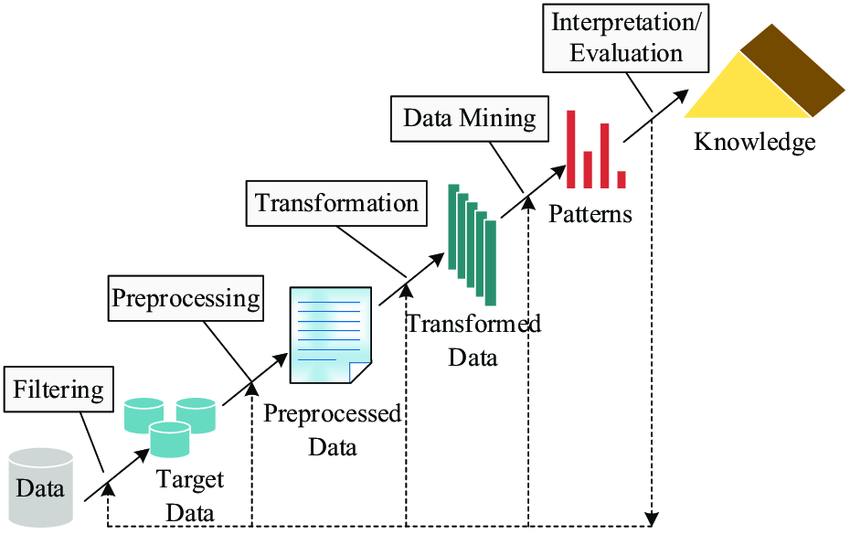
\includegraphics[width=0.65\textwidth]
    {figures/Data-mining-general-process.png}
    \caption{Sơ đồ quy trình KDD/Data Mining}
    \label{fig:data-mining-process}
\end{figure}
\clearpage

\subsection{Nhiệm vụ chi tiết từng bước}
\begin{enumerate}
    \item Làm sạch dữ liệu: Xử lý dữ liệu nhiễu, thiếu, sai sót.\\
    \textit{Ví dụ:} Điền giá trị trung bình vào các ô trống trong cột ``Tuổi''.

    \item Tích hợp dữ liệu: Hợp nhất dữ liệu từ nhiều nguồn khác nhau. \\
    \textit{Ví dụ:} Gộp bảng thông tin khách hàng và bảng lịch sử giao dịch.

    \item Trích chọn dữ liệu: Lấy ra tập dữ liệu con liên quan trực tiếp đến mục tiêu phân tích. \\
    \textit{Ví dụ:} Chỉ lấy dữ liệu khách hàng tại TP.HCM trong năm 2024.

    \item Chuyển đổi dữ liệu: Biến đổi dữ liệu về định dạng phù hợp cho thuật toán. \\
    \textit{Ví dụ:} Chuẩn hóa dữ liệu lương về đoạn $[0,1]$.

    \item Khai phá dữ liệu: Áp dụng các thuật toán thông minh để tìm mẫu. \\
    \textit{Ví dụ:} Dùng thuật toán Apriori tìm luật kết hợp, KNN để phân lớp.

    \item Đánh giá mẫu: Kiểm tra độ tin cậy và ý nghĩa của các mẫu tìm được.\\
    \textit{Ví dụ:} Loại bỏ các luật có độ tin cậy thấp, giữ lại luật giá trị.

    \item Biểu diễn tri thức: Trình bày kết quả cho người dùng cuối.\\
    \textit{Ví dụ:} Vẽ biểu đồ, bảng biểu, báo cáo trực quan.
\end{enumerate}

\subsection{Tiền xử lý dữ liệu và Trích xuất đặc trưng}
\textbf{Mục tiêu:} Giải quyết các vấn đề của dữ liệu thô như thiếu, nhiễu, trùng lặp, không nhất quán và quá nhiều chiều dữ liệu.

\subsubsection*{a. Tiền xử lý dữ liệu}
\begin{itemize}
    \item Feature Extraction: Tạo ra các đặc trưng có ý nghĩa từ dữ liệu thô.
    \item Feature Selection: Chọn lọc các đặc trưng quan trọng nhất ($k$ đặc trưng từ $n$ đặc trưng ban đầu), loại bỏ thông tin dư thừa.
    \item Feature Reduction: Giảm số chiều dữ liệu bằng cách biến đổi hoặc kết hợp đặc trưng.
    \item Normalization: Đưa các đặc trưng về cùng một khoảng giá trị (Min-Max hoặc Z-score).
\end{itemize}

\subsubsection*{b. Chi tiết về Giảm chiều dữ liệu}
\begin{enumerate}
    \item \textbf{Feature Selection}
    \begin{itemize}
        \item Khái niệm: Chọn ra tập con $k$ đặc trưng quan trọng nhất từ $n$ đặc trưng ban đầu ($k < n$), giữ nguyên ý nghĩa vật lý gốc.
        \item Ví dụ: Bộ dữ liệu bệnh tim có 20 chỉ số $\rightarrow$ Chỉ chọn 8 chỉ số quan trọng nhất để dự đoán.
    \end{itemize}

    \item \textbf{Feature Reduction}
    \begin{itemize}
        \item Khái niệm: Tạo ra các đặc trưng mới ít hơn số lượng ban đầu bằng cách chiếu dữ liệu sang không gian mới.
        \item Phương pháp phổ biến: PCA (Principal Component Analysis), SVD (Singular Value Decomposition).
    \end{itemize}

    \item \textbf{Thuật toán PCA}
    \begin{itemize}
        \item Định nghĩa: Phép biến đổi tuyến tính trực giao đưa các đặc trưng tương quan về các thành phần chính không tương quan.
        \item Mục đích: Giữ lại nhiều phương sai dữ liệu nhất khi giảm chiều
        \item Cơ sở toán học : Ma trận dữ liệu $X$ được phân rã thành: $X = U \Sigma V^T$.
        \item Các bước thực hiện PCA: (1) Chuẩn hóa dữ liệu; (2) Tính ma trận hiệp phương sai; (3) Tính trị riêng và vectơ riêng; (4) Chọn $k$ vectơ riêng ứng với trị riêng lớn nhất; (5) Chiếu dữ liệu ban đầu sang không gian mới tạo bởi các vectơ riêng này.
    \end{itemize}
\end{enumerate}

\subsection{Thực nghiệm PCA - Exercise 3.2.1}
\label{sec:pca321}
\subsubsection{Đề bài và dữ liệu đầu vào}
Theo bài Exercise 3.2.1 trong tài liệu hướng dẫn đã cung cấp : tạo hai bộ dữ liệu \(X_1\) và \(X_2\), mỗi bộ 400 vector ba chiều thuộc hai lớp, mỗi lớp 200 mẫu. Hai lớp có cùng ma trận hiệp phương sai:
\[
S=\begin{bmatrix}0.3&1.0&1.0\\1.0&9.0&1.0\\1.0&1.0&9.0\end{bmatrix}.
\]
\begin{itemize}
\item \textbf{Bộ \(X_1\):} \(m_1=(-6,6,6)^\top\), \(m_2=(6,6,6)^\top\).
\item \textbf{Bộ \(X_2\):} \(m_1=(-2,0,0)^\top\), \(m_2=(2,0,0)^\top\).
\end{itemize}
Yêu cầu: tính PCA và \textit{explained variance ratio}; chiếu dữ liệu lên hai thành phần chính đầu tiên; vẽ sáu đồ thị \(X_{11}\! -\! X_{12}\), \(X_{11}\! -\! X_{13}\), \(X_{12}\! -\! X_{13}\), \(Y_1\! -\! Y_2\), \(Y_1\! -\! Y_3\), \(Y_2\! -\! Y_3\) cho mỗi bộ; so sánh kết quả.
\subsubsection{Quy trình tính tay về mặt nguyên lý}
\begin{enumerate}
\item Lấy ma trận \(X\in\mathbb R^{400\times3}\), trong đó mỗi hàng là một vector dữ liệu. Lấy trung bình theo cột \(\bar x\), rồi tâm hóa \(X_c=X-\mathbf{1}\bar x^\top\).
\item Tính ma trận hiệp phương sai mẫu: \(\widehat S=\frac1{399}X_c^\top X_c\).
\item Tính trị riêng \(\lambda_1\ge\lambda_2\ge\lambda_3\) và vector riêng trực chuẩn \(v_1,v_2,v_3\) của \(\widehat S\).
\item Tỷ lệ phương sai của thành phần chính thứ \(j\): \(r_j=\lambda_j/(\lambda_1+\lambda_2+\lambda_3)\).
\item Chọn \(W_2=[v_1\ v_2]\). Dữ liệu sau giảm từ 3 còn 2 chiều: \(Z=X_cW_2\in\mathbb R^{400\times2}\). Khi cần vẽ đủ ba \(Y\), tạm giữ \(Y=X_c[v_1\ v_2\ v_3]\).
\end{enumerate}
\subsubsection{Kết quả chạy mã nguồn (seed = 42)}
Để có thể tái lập, dùng NumPy \texttt{default\_rng(42)}, sinh 200 mẫu mỗi lớp theo Gaussian nhiều chiều, sau đó \texttt{sklearn.decomposition.PCA} trên toàn bộ 400 mẫu \textit{không dùng nhãn lớp}. Kết quả thực thi:
\begin{center}\small\begin{tabular}{|l|r|r|r|r|}\hline
Tập&PC1 (\%)&PC2 (\%)&PC3 (\%)&PC1+PC2 (\%)\\\hline
X1&66.78&19.66&13.56&86.44\\\hline
X2&45.68&36.10&18.22&81.78\\\hline
\end{tabular}\end{center}
\noindent\textbf{Cách diễn giải:} Ví dụ tỷ lệ của \(X_1\) ở PC1 biểu thị phần phương sai dữ liệu được giữ lại khi chỉ chiếu lên vector riêng thứ nhất. Dùng hai PC sẽ giữ tổng tỷ lệ ở cột cuối. Đó là \textit{phương sai}, không trực tiếp là accuracy phân lớp.
\subsubsection{Mã nguồn Python thực nghiệm PCA}
\lstinputlisting[language=Python,caption={Mã nguồn chạy Exercise 3.2.1: tạo dữ liệu và biểu diễn 12 scatter plot.}]{source_code/pca_ex321.py}
\subsubsection{Các biểu đồ kết quả}
\noindent\textbf{Tập X1:} Các cặp tọa độ gốc (hàng trên) và sau biến đổi PCA (hàng dưới).
\begin{figure}[H]\centering
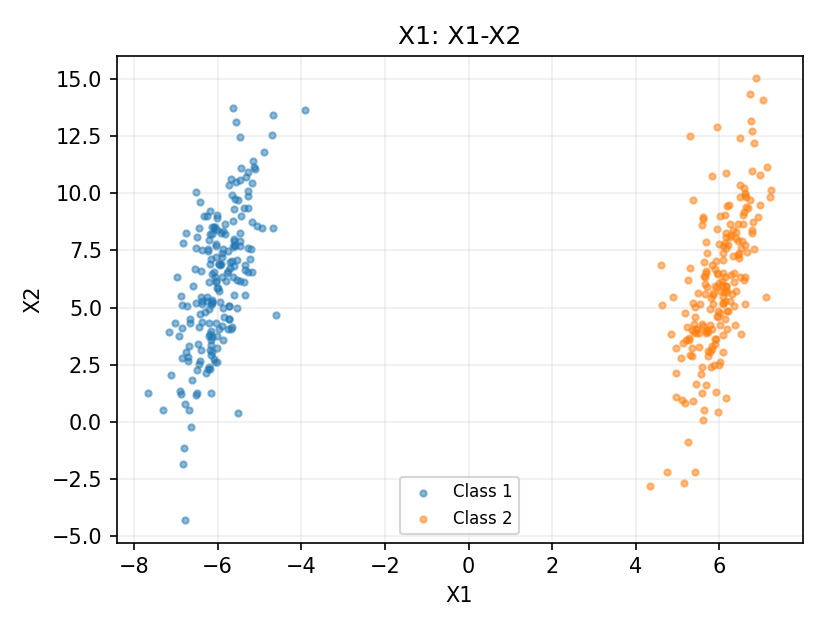
\includegraphics[width=0.315\linewidth]{figures/pca/X1_X1X2.png}\hfill
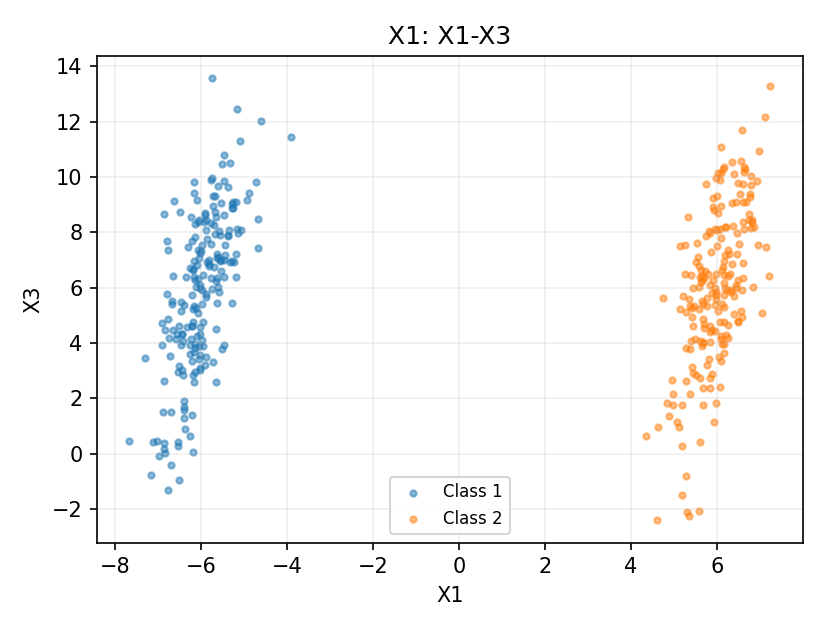
\includegraphics[width=0.315\linewidth]{figures/pca/X1_X1X3.png}\hfill
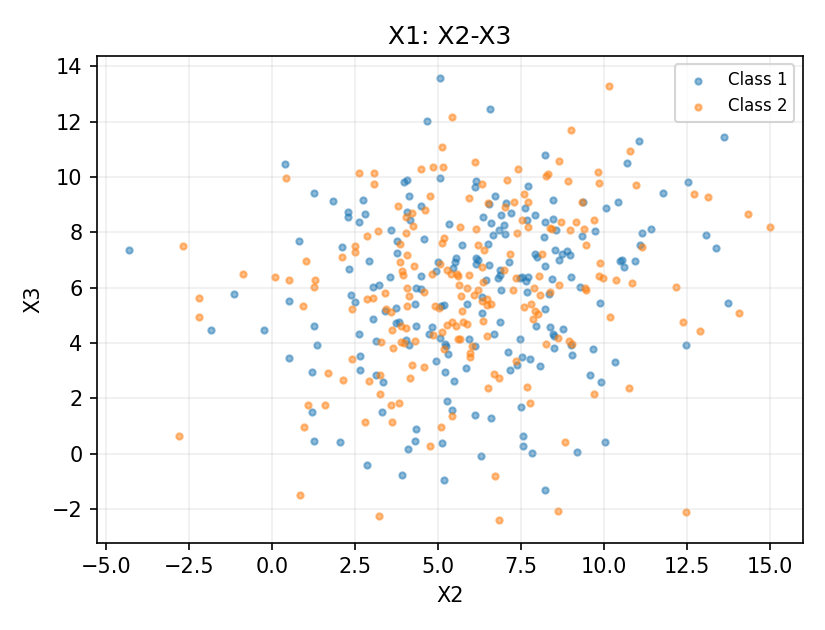
\includegraphics[width=0.315\linewidth]{figures/pca/X1_X2X3.png}\hfill
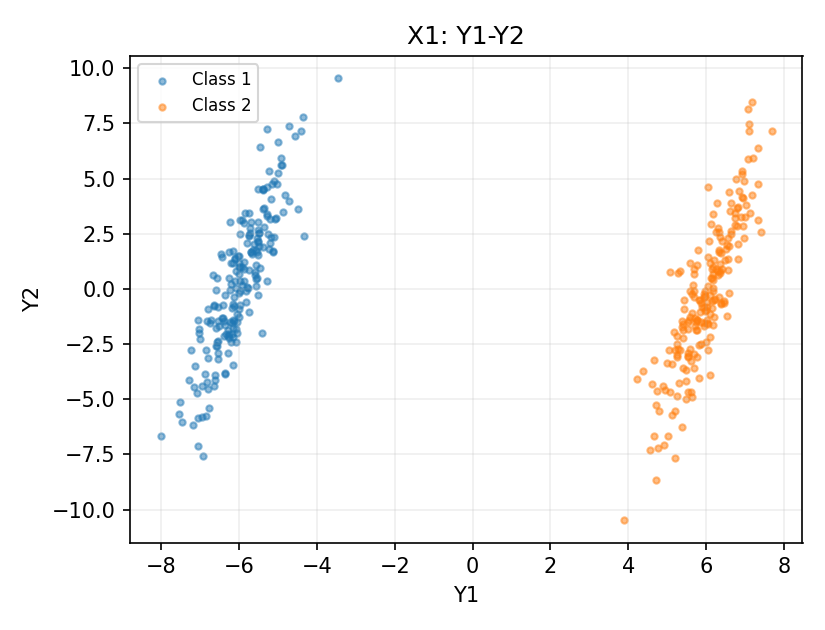
\includegraphics[width=0.315\linewidth]{figures/pca/X1_Y1Y2.png}\hfill
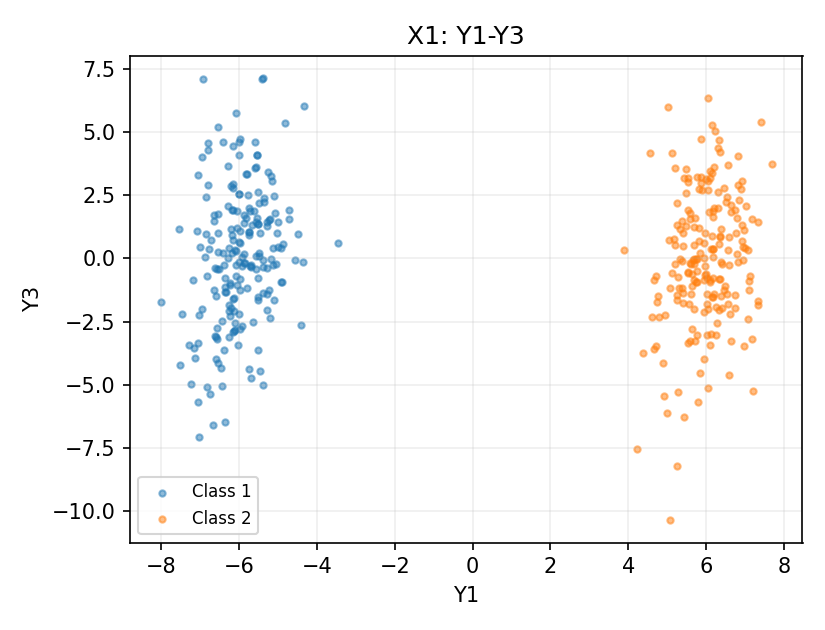
\includegraphics[width=0.315\linewidth]{figures/pca/X1_Y1Y3.png}\hfill
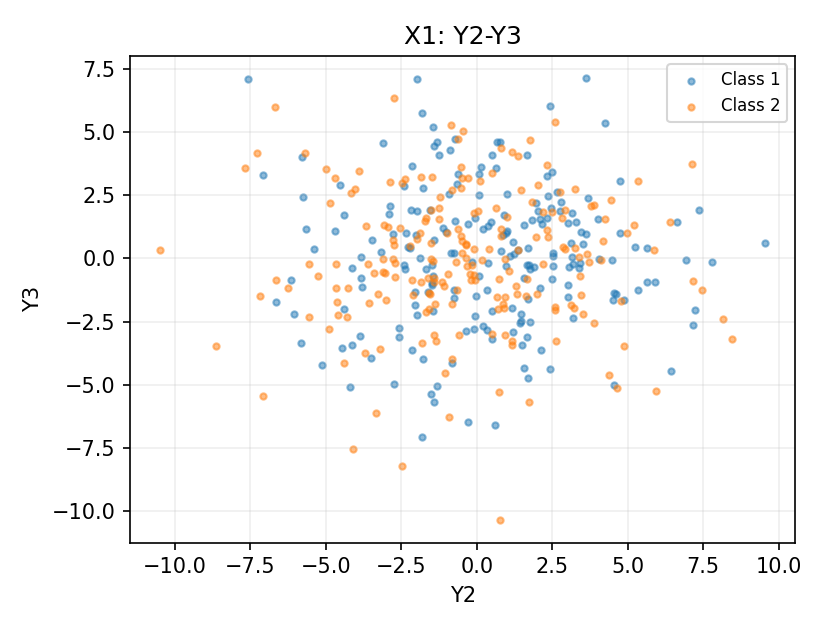
\includegraphics[width=0.315\linewidth]{figures/pca/X1_Y2Y3.png}\hfill
\caption{Sáu scatter plot của X1 theo yêu cầu Exercise 3.2.1.}
\end{figure}
\noindent\textbf{Tập X2:} Các cặp tọa độ gốc (hàng trên) và sau biến đổi PCA (hàng dưới).
\begin{figure}[H]\centering
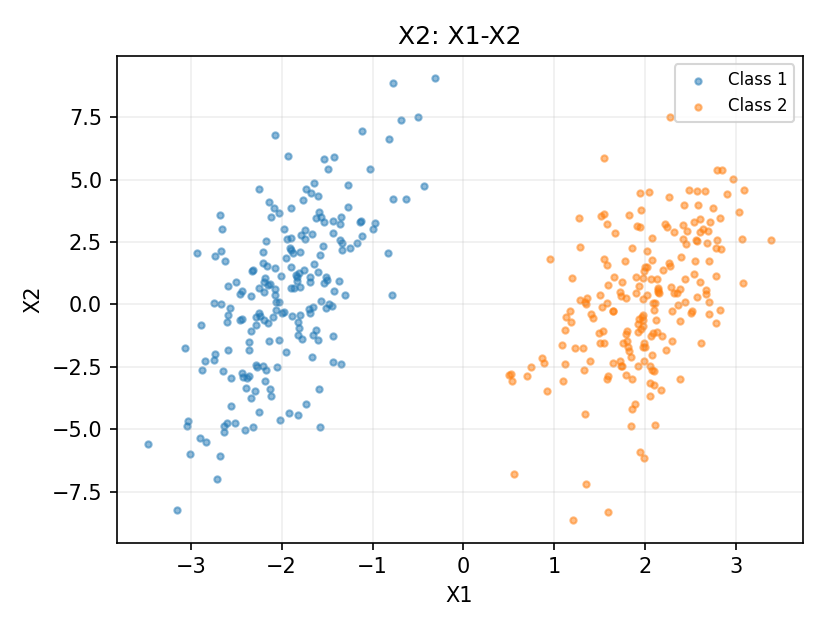
\includegraphics[width=0.315\linewidth]{figures/pca/X2_X1X2.png}\hfill
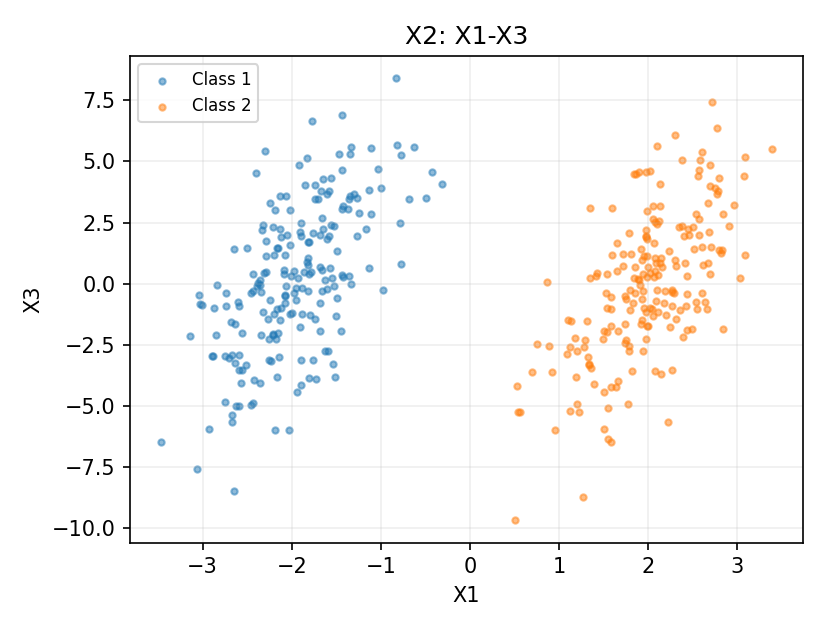
\includegraphics[width=0.315\linewidth]{figures/pca/X2_X1X3.png}\hfill
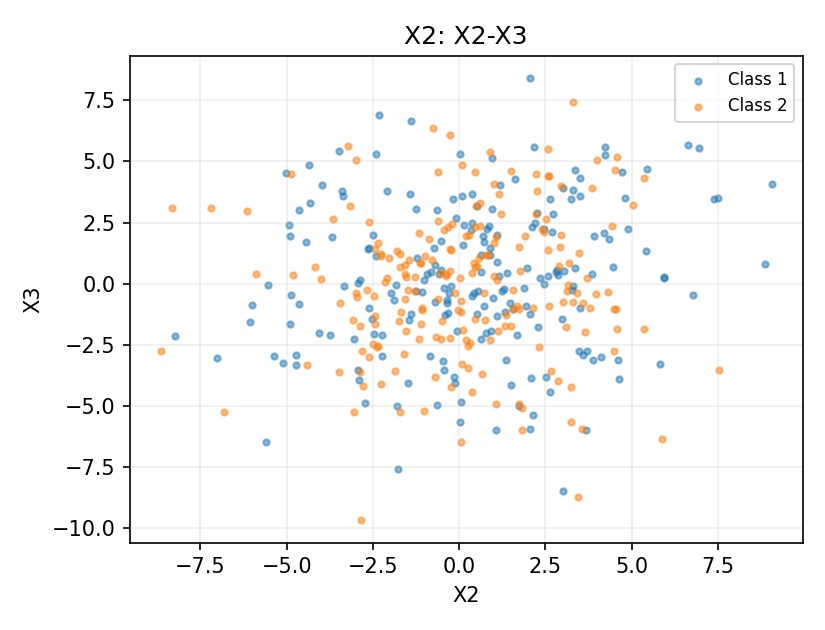
\includegraphics[width=0.315\linewidth]{figures/pca/X2_X2X3.png}\hfill
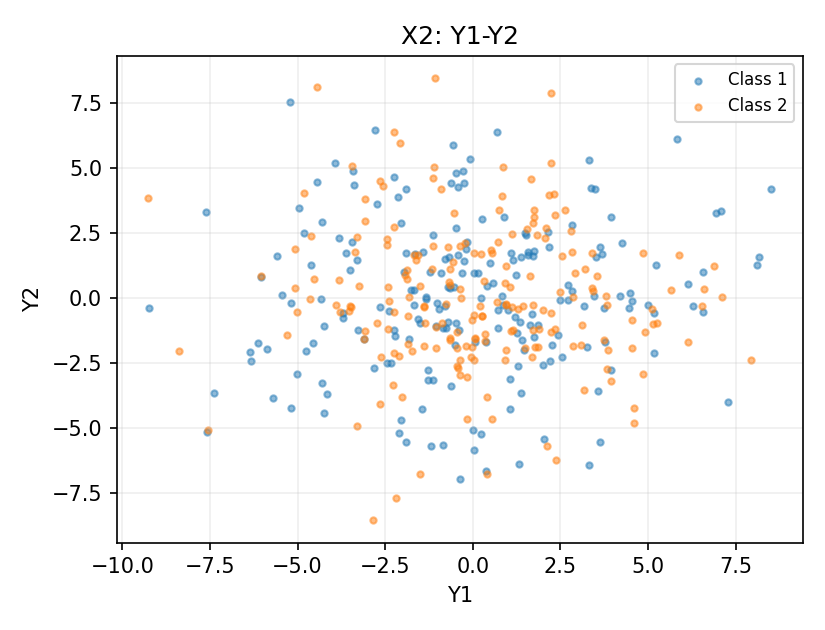
\includegraphics[width=0.315\linewidth]{figures/pca/X2_Y1Y2.png}\hfill
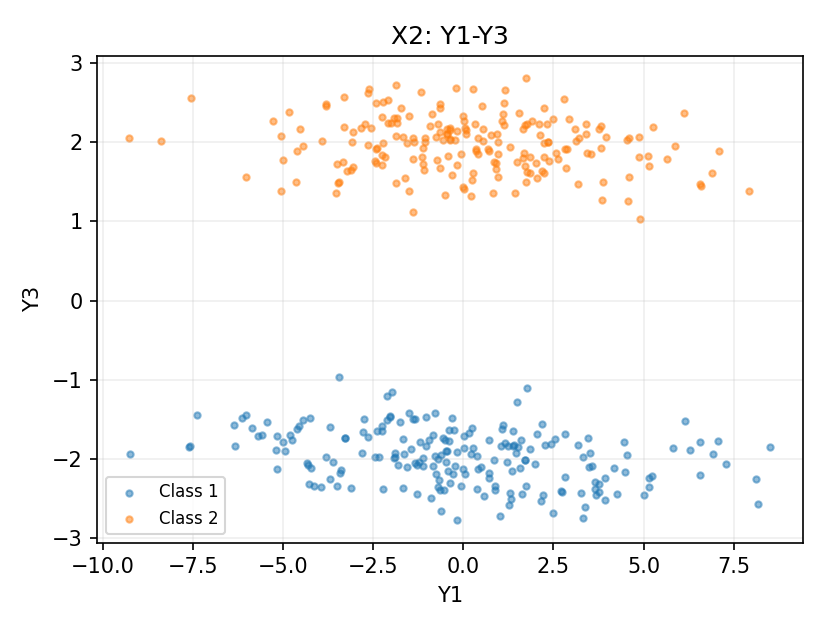
\includegraphics[width=0.315\linewidth]{figures/pca/X2_Y1Y3.png}\hfill
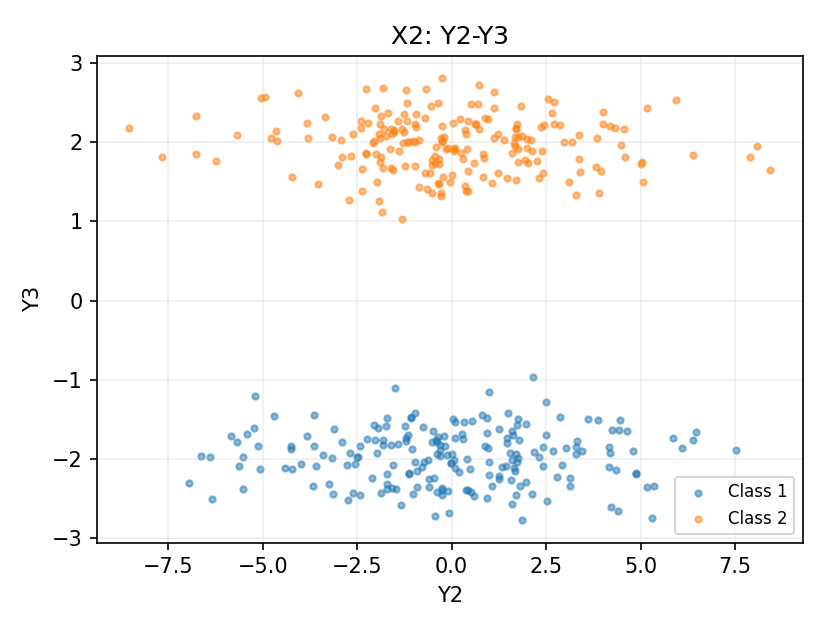
\includegraphics[width=0.315\linewidth]{figures/pca/X2_Y2Y3.png}\hfill
\caption{Sáu scatter plot của X2 theo yêu cầu Exercise 3.2.1.}
\end{figure}
\subsubsection{Nhận xét và kết luận}
\begin{itemize}
\item Ở \(X_1\), hai lớp lệch nhau rất rõ theo chiều thứ nhất, và PC1 giữ phần lớn phương sai vì còn có khác biệt trung bình giữa các lớp; giảm xuống 2 chiều vẫn thể hiện khá rõ sự tách biệt.
\item Ở \(X_2\), khoảng cách giữa hai trung bình lớp nhỏ hơn; PC1, PC2 chia sẻ phương sai tương đối đồng đều, và phép chiếu chỉ để bảo toàn phương sai không bảo đảm tối ưu khả năng phân lớp.
\item Kết quả phụ thuộc vào mẫu sinh ngẫu nhiên nên có thể khác các tỷ lệ trong ví dụ của sách; mọi số liệu ở bảng trên là kết quả chạy trực tiếp với seed 42, không sao chép từ ví dụ khác.
\end{itemize}

%\noindent\textbf{Mã nguồn tái lập:} \path{source_code/pca_ex321.py}; dữ liệu chiếu 2D xuất ra \path{figures/pca/X1_PCA_2D.csv} và \path{figures/pca/X2_PCA_2D.csv}.
\section{KHO DỮ LIỆU}

\subsection{Khái niệm}
Kho dữ liệu (Data Warehouse - DW) là tập hợp dữ liệu có đặc tính: Hướng chủ đề, Tích hợp, Ổn định và Biến thiên theo thời gian, nhằm mục đích hỗ trợ phân tích và ra quyết định quản trị.

\subsection{Phân biệt CSDL Tác nghiệp (OLTP) và Kho dữ liệu (OLAP)}
\begin{table}[H]
    \centering
    \renewcommand{\arraystretch}{1.3}
    \begin{tabularx}{\textwidth}{|p{2.8cm}|X|X|}
        \hline
        \textbf{Đặc điểm} & \textbf{CSDL Tác nghiệp (OLTP)} & \textbf{Kho dữ liệu (OLAP)} \\
        \hline
        \textbf{Mục đích} & Xử lý giao dịch hàng ngày & Phân tích, báo cáo, hỗ trợ ra quyết định chiến lược. \\
        \hline
        \textbf{Dữ liệu} & Dữ liệu hiện tại, chi tiết, cập nhật liên tục. & Dữ liệu lịch sử, tổng hợp, ít thay đổi. \\
        \hline
        \textbf{Thời gian} & Tốc độ xử lý giao dịch rất nhanh. & Truy vấn phân tích phức tạp, tốn nhiều thời gian hơn. \\   
        \hline
        \textbf{Cấu trúc} & Chuẩn hóa cao để tránh dư thừa. & Phi chuẩn hóa để tối ưu đọc. \\
        \hline
        \textbf{Thao tác} & Chủ yếu là Insert, Update, Delete. & Chủ yếu là Select, Aggregation. \\
        \hline
    \end{tabularx}
\end{table}

\subsection{Đặc tính cốt lõi của Kho dữ liệu}
\begin{enumerate}
    \item Hướng chủ đề: Dữ liệu được tổ chức theo các chủ đề chính (Khách hàng, Sản phẩm, Doanh thu...).
    \item Tích hợp: Dữ liệu được làm sạch và thống nhất từ nhiều nguồn khác nhau.
    \item Biến thiên theo thời gian: Luôn gắn liền với yếu tố thời gian.
    \item Ổn định/Bất biến: Dữ liệu sau khi đưa vào kho thường không bị sửa đổi hay ghi đè, chỉ đọc.
\end{enumerate}

\subsection{OLAP (Online Analytical Processing)}
\begin{itemize}
    \item Khái niệm: Công nghệ cho phép người dùng phân tích dữ liệu đa chiều một cách tương tác và nhanh chóng.
    \item Phân biệt: OLTP dùng để ghi dữ liệu (Insert/Update), OLAP dùng để đọc và phân tích đa chiều (Select/Aggregation).
    \item Ví dụ: Xem doanh thu theo Vùng miền và Thời gian.
\end{itemize}

\subsection{Kiến trúc Kho dữ liệu}
Kiến trúc bao gồm các thành phần chính: Nguồn dữ liệu; Trích xuất, Chuyển đổi và Tải dữ liệu; Kho dữ liệu trung tâm; Các kho dữ liệu nhỏ; Các công cụ phân tích dữ liệu.

\begin{figure}[H]
    \centering
    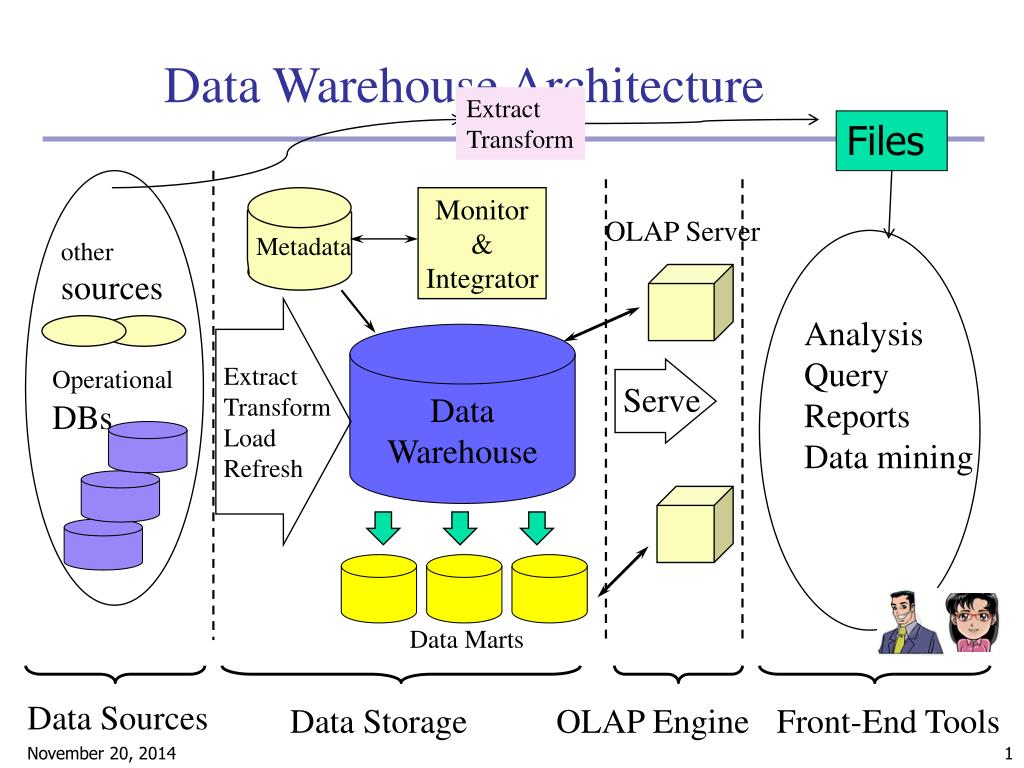
\includegraphics[width=1\textwidth]{figures/DW/Data_Warehouse.jpg}
    \caption{Kiến trúc Data Warehouse}
    \label{fig:data-warehouse}
\end{figure}

\subsection{Quy trình xây dựng}
Quy trình: (1) Xác định yêu cầu; (2) Thiết kế mô hình đa chiều; (3) ETL; (4) Triển khai; (5) Kiểm thử - bảo trì.

\subsection{Mô hình hóa Kho dữ liệu}
\begin{itemize}
    \item Mô hình Ngôi sao : Cấu trúc đơn giản nhất. Một bảng sự kiện Fact ở trung tâm, kết nối trực tiếp với các bảng chiều Dimension xung quanh. \textit{Ưu điểm:} Truy vấn cực nhanh, dễ hiểu.
    \item Mô hình Thiên hà : Đây là kiểu mô hình chứa vài bảng Fact và chia sẻ các bảng Dimension. \textit{Ưu điểm:} Giảm kích thước của cơ sở dữ liệu, tiết kiệm bộ nhớ.
    \item Mô hình Bông tuyết : Là dạng mở rộng của lược đồ hình sao bằng cách bổ sung các Dimension. Bảng Fact giống lược đồ hình sao. Bảng Dim được chuẩn hóa. Các chiều được cấu trúc rõ ràng. \textit{Ưu điểm:} Tiết kiệm bộ nhớ.
    \item Mô hình Chòm sao : Phức tạp nhất. Gồm nhiều bảng Fact chia sẻ chung bảng Dimension. \textit{Ứng dụng:} Hệ thống lớn.
\end{itemize}

\begin{figure}[H]
    \centering
    \begin{tabular}{cc}
        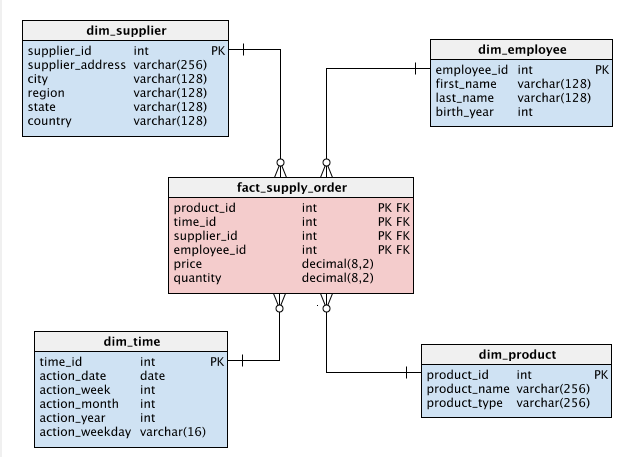
\includegraphics[width=0.45\textwidth,height=0.27\textheight,keepaspectratio]{figures/DW/Supply_Orders.png}
        &
        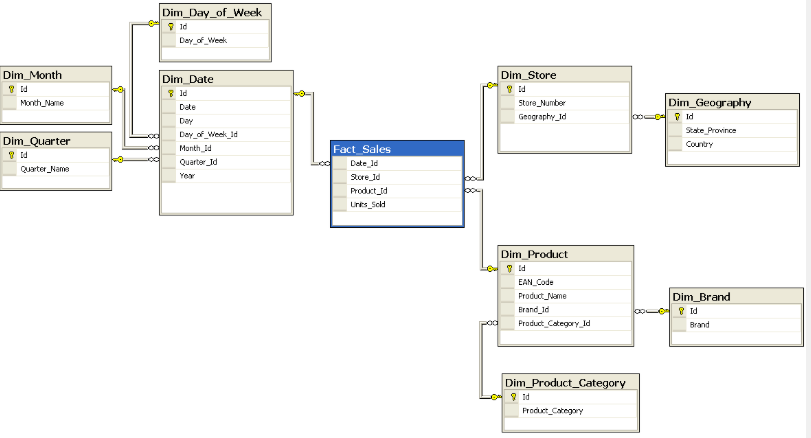
\includegraphics[width=0.45\textwidth,height=0.27\textheight,keepaspectratio]{figures/DW/Snowflake_Schema.png}
        \\
        \textbf{Mô hình Ngôi sao}
        &
        \textbf{Mô hình Bông tuyết}
        \\[0.8em]
        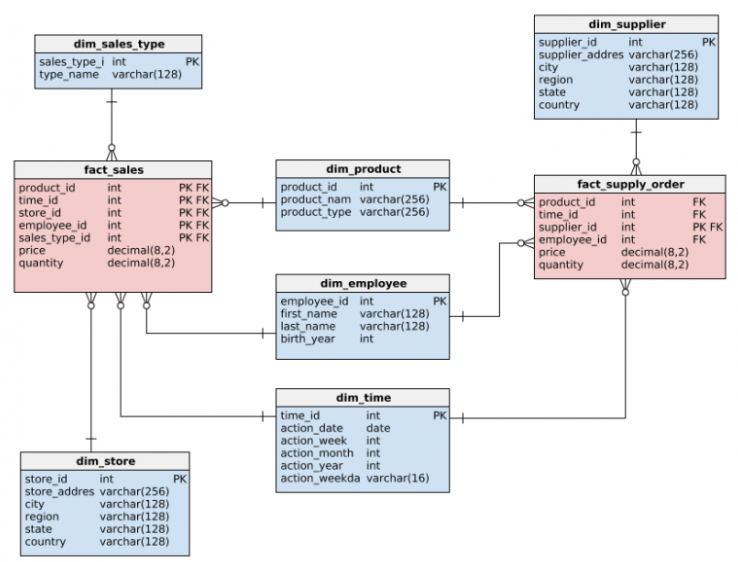
\includegraphics[width=0.45\textwidth,height=0.27\textheight,keepaspectratio]{figures/DW/Galaxy_Schema.png}
        &
        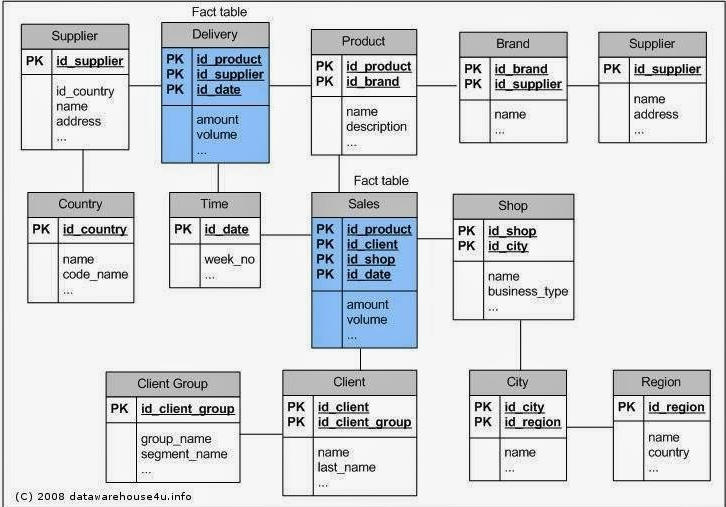
\includegraphics[width=0.45\textwidth,height=0.27\textheight,keepaspectratio]{figures/DW/Constellation_Schema.png}
        \\
        \textbf{Mô hình Thiên hà}
        &
        \textbf{Mô hình Chòm sao}
    \end{tabular}
\end{figure}

\section{HỌC MÁY (MACHINE LEARNING)}

\subsection{Khái niệm}
Là tập con của trí tuệ nhân tạo. Một lĩnh vực nhỏ của khoa học máy tính, nghiên cứu các thuật toán và mô hình thống kê cho phép máy tính thực hiện các nhiệm vụ mà không cần lập trình rõ ràng.

\subsection{Các cơ chế học}
\begin{enumerate}
    \item Supervised Learning: Dữ liệu huấn luyện có nhãn (Input $X$, Output $Y$). Ví dụ: Phân loại email spam.
    \item Unsupervised Learning: Dữ liệu không có nhãn, máy tự tìm cấu trúc. Ví dụ: Phân cụm khách hàng.
    \item Reinforcement Learning: Học thông qua thử-sai và nhận thưởng/phạt.
\end{enumerate}

\subsection{Liên hệ với Khai phá dữ liệu}
{\centering\fontsize{17}{21}\selectfont\bfseries\boldmath
$\text{Data Mining} = \text{ML} + \text{Database} + \text{Statistics}$. \par}
Học máy cung cấp các công cụ và thuật toán kỹ thuật để thực hiện các bước Khai phá dữ liệu. Data Mining chú trọng vào quy trình tìm tri thức, Machine Learning chú trọng vào thuật toán dự đoán/học.

\subsection{Ứng dụng của Học máy}
\begin{itemize}
    \item Nhận dạng hình ảnh và giọng nói.
    \item Phân loại văn bản, email spam.
    \item Trợ lý áo, chatbot.
    \item Hệ thống gợi ý.
    \item Chẩn đoán y tế, phát hiện gian lận.
\end{itemize}
\section{PHÂN LỚP}

\subsection{Khái niệm}
Là bài toán phân loại trong đó cho sẵn bộ dữ liệu huấn luyện được cấu thành từ 1 cặp (x,y), trong đó x là các thuộc tính và y là nhãn lớp từ đó xây dựng mô hình . Nhiệm vụ là dùng mô hình đó để phân loại nhãn lớp cho mẫu dữ liệu.

\subsection{Các thuật ngữ chuyên ngành}
\begin{table}[H]
    \centering
    \renewcommand{\arraystretch}{1.3}
    \begin{tabularx}{\textwidth}{|p{4.5cm}|X|}
        \hline
        \textbf{Thuật ngữ (Tiếng Anh)} & \textbf{Diễn giải (Tiếng Việt)} \\
        \hline
        Instance / Sample & Mẫu dữ liệu: Một đối tượng cụ thể hoặc một dòng trong bảng dữ liệu. \\
        \hline
        Label & Nhãn mục tiêu: Kết quả phân loại hoặc danh mục mẫu thuộc về. \\
        \hline
        Training dataset & Tập huấn luyện: Phần dữ liệu có nhãn dùng để ``dạy'' mô hình học. \\
        \hline
        Testing dataset & Tập kiểm thử: Phần dữ liệu đánh giá độ chính xác của mô hình sau khi học. \\
        \hline
        Feature extraction & Trích xuất đặc trưng: Kỹ thuật tạo đặc điểm mới từ dữ liệu thô. \\
        \hline
        Feature selection & Lựa chọn đặc trưng: Chọn lọc thuộc tính quan trọng nhất. \\
        \hline
        Feature reduction & Giảm chiều dữ liệu: Giảm bớt số lượng biến số đầu vào. \\
        \hline
        Ground truth & Giá trị thực tế: Đáp án đúng tuyệt đối để đối chiếu kết quả. \\
        \hline
    \end{tabularx}
\end{table}

\subsection{Quy trình phân lớp}
\begin{figure}[H]
    \centering
    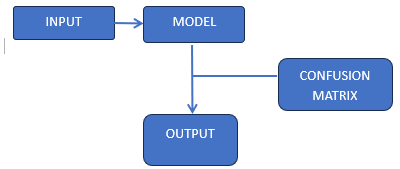
\includegraphics[width=1\textwidth]{figures/Classification/Classification_Process.png}
    \caption{Quy trình phân lớp}
    \label{fig:classification-process}
\end{figure}

Quy trình trong hình gồm hai giai đoạn. Ở giai đoạn huấn luyện, dữ liệu đã gán nhãn được tiền xử lý và dùng để xây dựng mô hình. Ở giai đoạn phân lớp, mô hình đã học nhận dữ liệu mới và dự đoán nhãn; nếu có nhãn thực tế, kết quả dự đoán được đối chiếu để đánh giá mô hình.

\subsection{Ví dụ và mô hình tổng quan}
\subsubsection*{5.1. Mô tả bài toán}
Xét bài toán dự đoán một học sinh có \textbf{đạt} bài kiểm tra hay không dựa trên hai thông tin: có đi học đầy đủ hay không và đã ôn bài hay chưa. Đây là bài toán phân lớp nhị phân với hai lớp \texttt{Yes} (đạt) và \texttt{No} (không đạt).

\subsubsection*{5.2. Mô tả dữ liệu}
Mỗi dòng là một mẫu học sinh. Hai cột ``Đi học đầy đủ'' và ``Ôn bài'' là các đặc trưng (features); cột ``Đạt bài kiểm tra'' là nhãn lớp (label). Bộ dữ liệu huấn luyện minh họa gồm ba mẫu:

\begin{table}[H]
    \centering
    \renewcommand{\arraystretch}{1.2}
    \begin{tabular}{|c|c|c|c|}
        \hline
        \textbf{Mẫu} & \textbf{Đi học đầy đủ} & \textbf{Ôn bài} & \textbf{Đạt bài kiểm tra (nhãn)} \\
        \hline
        1 & Yes & Yes & Yes \\
        \hline
        2 & Yes & No  & Yes \\
        \hline
        3 & No  & No  & No \\
        \hline
    \end{tabular}
    \caption{Ba mẫu dữ liệu huấn luyện cho ví dụ phân lớp}
    \label{tab:classification-simple-example}
\end{table}

\begin{figure}[H]
    \centering
    \begin{tikzpicture}[
        node distance=0.75cm and 0.8cm,
        box/.style={draw, rounded corners, align=center, minimum width=3.1cm, minimum height=1.05cm},
        arrow/.style={->, thick}
    ]
        \node[box] (data) {Dữ liệu huấn luyện\\3 mẫu, 2 đặc trưng, nhãn Yes/No};
        \node[box, right=of data] (train) {Huấn luyện\\mô hình phân lớp};
        \node[box, right=of train] (model) {Mô hình\\phân lớp};
        \node[box, below=of model] (predict) {Dự đoán nhãn\\Yes hoặc No};
        \node[box, left=of predict] (new) {Mẫu mới\\Đi học: Yes; Ôn bài: Yes};
        \draw[arrow] (data) -- node[above, align=center] {Học từ mẫu\\đã có nhãn} (train);
        \draw[arrow] (train) -- (model);
        \draw[arrow] (predict) -- (new);
        \draw[arrow] (model.south) -- ++(0,-0.35) -| node[pos=0, below] {áp dụng mô hình} (predict.north);
    \end{tikzpicture}
    \caption{Mô hình tổng quan của ví dụ phân lớp học sinh đạt hay không đạt}
    \label{fig:classification-simple-example}
\end{figure}
\subsubsection*{5.3. Nhiệm vụ phân lớp}
Từ ba mẫu đã biết nhãn, xây dựng mô hình học mối liên hệ giữa hai đặc trưng và kết quả kiểm tra. Sau đó, đưa đặc trưng của một học sinh mới vào mô hình để dự đoán nhãn \texttt{Yes} (đạt) hoặc \texttt{No} (không đạt). Với bảng minh họa trên, mẫu mới có ``Đi học đầy đủ = Yes'' và ``Ôn bài = Yes''; mô hình có thể dự đoán \texttt{Yes}.
\section{THUẬT TOÁN K-NN}

\subsection{Khái niệm}
- Là 1 thuật toán học máy có giám sát thường được sử dụng để phân loại.\\
- Hoạt động bằng cách tìm các điểm dữ liệu gần nhất “k”(hàng xóm) với 1 đầu vào nhất định và đưa ra dự đoán dựa trên lớp đa số hoặc giá trị trung bình.

\subsection{Các tham số cốt lõi}
Để vận hành K-NN, ta cần quan tâm hai yếu tố chính:
\begin{itemize}
    \item Tham số $k$ :
    \begin{itemize}
        \item Đây là tham số quyết định số lượng điểm hàng xóm tham gia vào việc bỏ phiếu.
        \item Lựa chọn $k$: Nếu $k$ quá nhỏ (ví dụ $k=1$), mô hình rất nhạy cảm với nhiễu. Nếu $k$ quá lớn, ranh giới phân lớp sẽ bị làm mờ, dẫn đến độ chính xác cục bộ giảm.
    \end{itemize}
    \item Độ đo khoảng cách :
    \begin{itemize}
        \item Để biết đâu là "hàng xóm gần nhất", ta cần thước đo. Phổ biến nhất là Khoảng cách Euclid (Euclidean Distance) - đoạn thẳng nối hai điểm trong không gian hình học.
        \item Công thức tổng quát giữa hai điểm $P$ và $Q$ trong không gian $n$ chiều:
        $$d(P,Q) = \sqrt{\sum_{i=1}^{n}(p_i - q_i)^2}$$
        Trong đó: $p_i$ và $q_i$ lần lượt là giá trị tọa độ (thuộc tính) thứ $i$ của hai điểm dữ liệu.
    \end{itemize}
\end{itemize}

\subsection{Quy trình thực hiện thuật toán}
Quy trình hoạt động của K-NN được chia thành 4 bước tuần tự:
\begin{itemize}
    \item \textbf{Bước 1:} Chuẩn bị tập huấn luyện có đặc trưng và nhãn; tách riêng tập kiểm thử.
    \item \textbf{Bước 2:} Tính khoảng cách từ điểm dữ liệu mới đến tất cả các điểm trong tập huấn luyện.
    \item \textbf{Bước 3:} Sắp xếp các điểm theo khoảng cách tăng dần và xác định $k$ điểm gần nhất.
    \item \textbf{Bước 4:} Dự đoán nhãn cho điểm dữ liệu mới dựa trên nhãn của $k$ điểm gần nhất (bỏ phiếu đa số).
\end{itemize}

\subsection{Mã giả thuật toán}
\begin{lstlisting}[caption={Mã giả thuật toán KNN}]
Algorithm KNN_Prediction:
Input:
    Du lieu Training (X_train, y_train)
    Diem du lieu moi can du doan (x_new)
    Tham so k 
Begin:
    1. Khoi tao danh sach luu tru khoang cach (Distances_List)
    2. Lap qua tung diem du lieu (x_i) trong X_train:
       a. Tinh khoang cach d = Euclidean(x_i, x_new)
       b. Them d vao Distances_List
    3. Sap xep Distances_List theo chieu tang dan.
    4. Chon ra k diem co khoang cach nho nhat (Top k neighbors).
    5. Thong ke nhan cua k diem nay.
    6. Return : Nhan co tan suat xuat hien cao nhat.
End
\end{lstlisting}

\subsection{Ví dụ minh họa chi tiết}
\textbf{Training dataset:}
\begin{table}[H]
    \centering
    \begin{tabular}{|c|c|c|c|}
        \hline
        \textbf{ID} & \textbf{Feature 1} & \textbf{Feature 2} & \textbf{Class} \\
        \hline
        1 & 3 & 4 & A \\ \hline
        2 & 1.5 & 5 & A \\ \hline
        3 & 6 & 8 & A \\ \hline
        4 & 2.5 & 5 & A \\ \hline
        5 & 5 & 2.5 & B \\ \hline
        6 & 5 & 2 & B \\ \hline  
        7 & 8 & 3 & B \\ \hline
        8 & 4.5 & 3 & B \\ \hline
    \end{tabular}
\end{table}

\textbf{Testing dataset} (Size: 10 instances, 2 features, 2 classes):
\begin{table}[H]
    \centering
    \begin{tabular}{|c|c|c|c|}
        \hline
        \textbf{ID} & \textbf{Feature 1} & \textbf{Feature 2} & \textbf{Class} \\
        \hline
        9 & 8 & 1.5 & ? \\ \hline
        10 & 4.5 & 7 & ? \\ \hline
    \end{tabular}
\end{table}

\begin{itemize}
    \item Tính toán cho Test point 9 $(8, 1.5)$ với $k=3$: Sau khi tính khoảng cách và xếp hạng (Rank), 3 láng giềng gần nhất là các mẫu có ID 7, 6, 5 (đều thuộc Class B). $\rightarrow$ \textbf{Kết quả:} Test point 9 có class B.
    \item Tính toán cho Test point 10 $(4.5, 7)$ với $k=3$: Sau khi tính khoảng cách và xếp hạng (Rank), 3 láng giềng gần nhất là các mẫu có ID 3, 8, 7 (đều thuộc Class A). $\rightarrow$ Kết quả: Test point 10 có class A.
\end{itemize}

\subsection{Chương trình cho bài toán minh họa}
\lstinputlisting[language=Python,caption={Chương trình Python minh họa thuật toán KNN}]{source_code/knn66.py}

\subsection{Ưu/nhược điểm thuật toán K-NN}
\begin{itemize}
    \item \textbf{Ưu điểm:}
    \begin{itemize}
        \item \textit{Không yêu cầu mô hình phức tạp:} K-NN không yêu cầu xây dựng mô hình trước mà sử dụng dữ liệu trực tiếp để phân loại.
        \item \textit{Đơn giản và dễ hiểu:} Thuật toán rất đơn giản để triển khai và trực quan, đặc biệt khi dữ liệu ít thuộc tính.
        \item \textit{Tận dụng tính cục bộ:} Có khả năng mô tả tốt các đặc điểm cục bộ vì dựa trên những điểm gần nhất.
    \end{itemize}
    \item \textbf{Nhược điểm:}
    \begin{itemize}
        \item \textit{Tốc độ chậm:} Có thể chậm trong giai đoạn phân loại khi dữ liệu lớn vì phải tính khoảng cách đến tất cả các mẫu.
        \item \textit{Dễ bị ảnh hưởng bởi nhiễu:} Các điểm dữ liệu nhiễu hoặc thuộc tính không liên quan làm giảm độ chính xác.
        \item \textit{Yêu cầu bộ nhớ lớn:} Cần lưu giữ toàn bộ tập dữ liệu huấn luyện để phân loại.
    \end{itemize}
\end{itemize}
\section{THUẬT TOÁN NAIVE BAYES}

\subsection{Khái niệm}
Naive Bayes là một thuật toán phân lớp dựa trên định lý Bayes với giả định độc lập giữa các thuộc tính. Thuật toán này sử dụng xác suất để đoán nhãn của một mẫu mới dựa trên phân phối xác suất của các nhãn và giá trị của các thuộc tính trong tập huấn luyện.

Định lý Bayes:
$$P(A\vert{}B) = \frac{P(B\vert{}A)P(A)}{P(B)}$$

Trong đó:
\begin{itemize}
    \item $P(A\vert{}B)$: Xác suất của sự kiện $A$ xảy ra khi biết sự kiện $B$ đã xảy ra (gọi là xác suất có điều kiện).
    \item $P(B\vert{}A)$: Xác suất của sự kiện $B$ xảy ra khi biết sự kiện $A$ đã xảy ra.
    \item $P(A)$: Xác suất tiên nghiệm của sự kiện $A$ (xác suất xảy ra của $A$ mà không cần biết gì về $B$).
    \item $P(B)$: Xác suất tiên nghiệm của sự kiện $B$.
\end{itemize}

\subsection{Quy trình thực hiện}
\begin{itemize}
    \item \textbf{Bước 1:} Xác định các nhãn lớp và các thuộc tính từ tập dữ liệu huấn luyện.
    \item \textbf{Bước 2:} Tính xác suất tiên nghiệm $P(c)$ cho mỗi nhãn $c$.
    \item \textbf{Bước 3:} Tính xác suất có điều kiện $P(x\vert{}c)$ cho từng thuộc tính $x_i$ và nhãn $c$.
    \item \textbf{Bước 4:} Áp dụng công thức Bayes tính xác suất hậu nghiệm:
    $$P(c\vert{}x) = \frac{P(x\vert{}c)P(c)}{P(x)}$$
    \item \textbf{Bước 5:} Dự đoán nhãn có xác suất lớn nhất.
\end{itemize}

\subsection{Mã giả}
\begin{lstlisting}[caption={Mã giả thuật toán Naïve Bayes}]
Algorithm Naive_Bayes_Prediction:
1. Input: Training dataset, Test dataset
2. For each class C in Training dataset:
3.     Compute P(C)
4.     For each attribute x_i in X:
5.         Compute P(x_i | C)
6. For each sample X in Test dataset:
7.     Compute P(C|X) = P(C) * Product(P(x_i | C) for all x_i in X)
8.     Assign X to the class C with the highest P(C|X)
9. Output: Predicted labels
\end{lstlisting}

\subsection{Ví dụ minh họa chi tiết}

Tập huấn luyện có 14 mẫu, với 9 mẫu \textit{Yes}, 5 mẫu \textit{No}.
Xét mẫu cần phân loại gồm bốn thuộc tính:
\[X=(\mathrm{Sunny},\mathrm{Cool},\mathrm{High},\mathrm{True}).\]
\begin{table}[H]
    \centering
    \small
    \renewcommand{\arraystretch}{1.15}
    \begin{tabular}{|c|c|c|c|c|c|}
        \hline
        \rowcolor{yellow}
        \textbf{ID} & \textbf{Outlook} & \textbf{Temp} & \textbf{Humidity} & \textbf{Windy} & \textbf{Play} \\
        \hline
        1 & Sunny & Hot & High & False & No \\
        \hline
        2 & Sunny & Hot & High & True & No \\
        \hline
        3 & Overcast & Hot & High & False & Yes \\
        \hline
        4 & Rainy & Mild & High & False & Yes \\
        \hline
        5 & Rainy & Cool & Normal & False & Yes \\
        \hline
        6 & Rainy & Cool & Normal & True & No \\
        \hline
        7 & Overcast & Cool & Normal & True & Yes \\
        \hline
        8 & Sunny & Mild & High & False & No \\
        \hline
        9 & Sunny & Cool & Normal & False & Yes \\
        \hline
        10 & Rainy & Mild & Normal & False & Yes \\
        \hline
        11 & Sunny & Mild & Normal & True & Yes \\
        \hline
        12 & Overcast & Mild & High & True & Yes \\
        \hline
        13 & Overcast & Hot & Normal & False & Yes \\
        \hline
        14 & Rainy & Mild & High & True & No \\
        \hline
        \rowcolor{yellow}
        15 & Sunny & Cool & High & True & ??? \\
        \hline
    \end{tabular}
    \caption{Tập dữ liệu Play Tennis và mẫu cần phân loại}
    \label{tab:naive-bayes-play-tennis}
\end{table}
\subsubsection{Bước 1. Xác suất tiên nghiệm}
\[
P(\mathrm{Yes})=\frac{9}{14},\qquad P(\mathrm{No})=\frac{5}{14}.
\]
\subsubsection{Bước 2. Xác suất điều kiện}
\begin{center}\small
\begin{tabular}{@{}lcc@{}}\toprule
Giá trị đặc trưng&$P(\cdot\mid\mathrm{Yes})$&$P(\cdot\mid\mathrm{No})$\\\midrule
Outlook = Sunny&$2/9$&$3/5$\\
Temperature = Cool&$3/9$&$1/5$\\
Humidity = High&$3/9$&$4/5$\\
Windy = True&$3/9$&$3/5$\\\bottomrule
\end{tabular}\end{center}
\subsubsection{Bước 3. Tính xác suất hậu nghiệm}
\begin{align*}
P(\mathrm{Yes}\vert{}x)&=\frac9{14}\frac29\frac39\frac39\frac39\approx 0.00529,\\
P(\mathrm{No}\vert{}x)&=\frac5{14}\frac35\frac15\frac45\frac35\approx 0.02057.
\end{align*}
\subsubsection{Bước 4. Kết luận}
Vì $P(\mathrm{No}\vert{}x)>P(\mathrm{Yes}\vert{}x)$, mẫu được dự đoán là \textbf{No}.

\subsection{Viết chương trình cho bài toán được minh họa}
\lstinputlisting[language=Python,caption={Chương trình Python minh họa thuật toán Naive Bayes}]{source_code/naive_bayes_75.py}

\subsection{Ưu/nhược điểm của thuật toán Naive Bayes}
\begin{itemize}
    \item \textbf{Ưu điểm:}
    \begin{itemize}
        \item Hiệu quả với dữ liệu lớn và nhiều thuộc tính.
        \item Đơn giản, dễ hiểu, dễ triển khai.
        \item Thích hợp cho các bài toán phân loại văn bản như phân loại email hoặc phân tích cảm xúc.
    \end{itemize}
    \item \textbf{Nhược điểm:}
    \begin{itemize}
        \item Giả định độc lập giữa các thuộc tính thường không đúng trong thực tế, có thể làm giảm độ chính xác.
        \item Không hiệu quả khi dữ liệu có giá trị bằng 0 trong các xác suất.
    \end{itemize}
\end{itemize}
\section{THUẬT TOÁN DECISION TREE}

\subsection{Khái niệm}
Decision Tree (Cây quyết định) là mô hình phân lớp (hoặc hồi quy) dạng cây, trong đó:
\begin{itemize}
    \item Nút trong: tương ứng với một thuộc tính dùng để tách dữ liệu.
    \item Cạnh: tương ứng với giá trị của thuộc tính đó.
    \item Nút lá: tương ứng với nhãn lớp được dự đoán.
\end{itemize}

Ý tưởng chính của thuật toán Decision Tree: Chia để trị. Tại mỗi bước, chọn thuộc tính tốt nhất để tách dữ liệu thành các nhánh con sao cho các mẫu trong cùng một nhánh có cùng nhãn lớp càng nhiều càng tốt.

\subsection{Quy trình phân lớp bằng thuật toán Decision Tree (ID3)}
Quy trình chung:
\begin{enumerate}[label=\textbf{Bước \arabic*:}]
  \item Chuẩn bị và làm sạch dữ liệu.
  \item Tại tập $S$ hiện thời, tính độ bất định (Entropy) và đánh giá các thuộc tính.
  \item Chọn thuộc tính có Information Gain lớn nhất (ID3); với C4.5 sử dụng Gain Ratio.
  \item Tách tập theo thuộc tính được chọn rồi gọi đệ quy cho từng nhánh.
  \item Dừng khi các mẫu đồng nhất nhãn hoặc hết điều kiện chia; cắt tỉa nếu cần.
\end{enumerate}
\begin{align}
H(S)&=-\sum_{c}p(c)\log_2p(c),\\
\operatorname{Gain}(S,A)&=H(S)-\sum_{v\in\operatorname{Values}(A)}\frac{|S_v|}{|S|}H(S_v),\\
\operatorname{Gini}(S)&=1-\sum_c p(c)^2.
\end{align}

\subsection{Mã giả}
\begin{lstlisting}[caption={Mã giả thuật toán ID3}]
ID3(S, Attributes)
Input:
    S: tap mau huan luyen
    Attributes: danh sach thuoc tinh con lai co the tach
Output:
    Mot cay quyet dinh

1. Neu tat ca mau trong S thuoc cung mot lop C:
       Tra ve nut la gan nhan C
2. Neu Attributes rong:
       Tra ve nut la voi nhan = lop xuat hien nhieu nhat trong S
3. Tinh Entropy(S)
4. Voi moi thuoc tinh A trong Attributes:
       Tinh Gain(S, A)
5. Chon A* = thuoc tinh co Gain(S, A) lon nhat
6. Tao nut N tuong ung voi thuoc tinh A*
7. Voi moi gia tri v cua A*:
       S_v = tap con cua S voi A* = v
       Neu S_v rong:
           Tao nut la con cua N, gan nhan = lop da so trong S
       Nguoc lai:
           Gan nhanh con cho N la ket qua goi de quy ID3(S_v, Attributes \ {A*})
8. Tra ve nut N
\end{lstlisting}

\subsection{Ví dụ minh họa - Tính tay chi tiết}

\subsubsection*{Mô tả bài toán}
Bài toán: Dựa vào điều kiện thời tiết, ta quyết định ``Có nên chơi tennis hay không''. \\
Lớp: $\text{PlayTennis} \in \{\text{Yes}, \text{No}\}$. \\
Mục tiêu: từ dữ liệu quá khứ, xây cây quyết định giúp dự đoán chơi / không chơi.

\subsubsection*{Mô tả dữ liệu}
Bảng dữ liệu (14 mẫu kinh điển - PlayTennis):
\begin{table}[H]
    \centering
    \begin{tabular}{|c|c|c|c|c|c|}
        \hline
        \textbf{No} & \textbf{Outlook} & \textbf{Temperature} & \textbf{Humidity} & \textbf{Wind} & \textbf{PlayTennis} \\
        \hline
        1 & Sunny & Hot & High & Weak & No \\ \hline
        2 & Sunny & Hot & High & Strong & No \\ \hline
        3 & Overcast & Hot & High & Weak & Yes \\ \hline
        4 & Rain & Mild & High & Weak & Yes \\ \hline
        5 & Rain & Cool & Normal & Weak & Yes \\ \hline
        6 & Rain & Cool & Normal & Strong & No \\ \hline
        7 & Overcast & Cool & Normal & Strong & Yes \\ \hline
        8 & Sunny & Mild & High & Weak & No \\ \hline
        9 & Sunny & Cool & Normal & Weak & Yes \\ \hline
        10 & Rain & Mild & Normal & Weak & Yes \\ \hline
        11 & Sunny & Mild & Normal & Strong & Yes \\ \hline
        12 & Overcast & Mild & High & Strong & Yes \\ \hline
        13 & Overcast & Hot & Normal & Weak & Yes \\ \hline
        14 & Rain & Mild & High & Strong & No \\ \hline
    \end{tabular}
    \caption{Dữ liệu PlayTennis (Tổng: 14 mẫu -- Yes: 9, No: 5)}
\end{table}

\subsubsection*{Tính tay từng bước theo quy trình ID3}
\textbf{Bước 1.} Entropy toàn bộ tập $S$: Tập $S$ có 9 Yes và 5 No:
$$\text{Entropy}(S) = -\left(\frac{9}{14}\right)\log_2\left(\frac{9}{14}\right) - \left(\frac{5}{14}\right)\log_2\left(\frac{5}{14}\right) \approx 0.940$$

\textbf{Bước 2.} Tính Information Gain cho từng thuộc tính: Ta xét 4 thuộc tính: Outlook, Temperature, Humidity, Wind.
\begin{itemize}
    \item 2.1. Thuộc tính Outlook (Sunny, Overcast, Rain):
    \begin{itemize}
        \item Sunny: (Mẫu 1, 2, 8, 9, 11) $\rightarrow$ 2 Yes, 3 No. $\text{Entropy}(\text{Sunny}) \approx 0.971$
        \item Overcast: (Mẫu 3, 7, 12, 13) $\rightarrow$ 4 Yes, 0 No. $\text{Entropy}(\text{Overcast}) = 0$
        \item Rain: (Mẫu 4, 5, 6, 10, 14) $\rightarrow$ 3 Yes, 2 No. $\text{Entropy}(\text{Rain}) \approx 0.971$
        $$\text{Gain}(S, \text{Outlook}) = 0.940 - \left[\frac{5}{14}(0.971) + \frac{4}{14}(0) + \frac{5}{14}(0.971)\right] \approx 0.246$$
    \end{itemize}
    \item 2.2. Thuộc tính Temperature: $\text{Gain}(S, \text{Temperature}) \approx 0.029$
    \item 2.3. Thuộc tính Humidity: $\text{Gain}(S, \text{Humidity}) \approx 0.152$
    \item 2.4. Thuộc tính Wind: $\text{Gain}(S, \text{Wind}) \approx 0.048$
\end{itemize}
\textbf{Kết luận:} Outlook có Information Gain lớn nhất $\rightarrow$ chọn Outlook làm nút gốc.

\subsubsection*{Xây tiếp các nhánh con}
\begin{itemize}
    \item Nhánh 1: $\text{Outlook} = \text{Overcast}$: Những mẫu có $\text{Outlook} = \text{Overcast}$ đều $\text{PlayTennis} = \text{Yes}$ (4 mẫu). $\text{Entropy} = 0 \rightarrow$ nút lá: Yes.
    \item Nhánh 2: $\text{Outlook} = \text{Sunny}$: Tập con Sunny (Mẫu 1, 2, 8, 9, 11) có 2 Yes, 3 No. $\text{Entropy} \approx 0.971$. Tính Gain cho các thuộc tính còn lại:
    \begin{itemize}
        \item $\text{Gain}(\text{Sunny}, \text{Humidity}) \approx 0.971$ (Lớn nhất) $\rightarrow$ Chọn Humidity làm nút con.
        \item $\text{Humidity} = \text{High}$: (Mẫu 1, 2, 8) $\rightarrow$ Tất cả No $\rightarrow$ Lá: No.
        \item $\text{Humidity} = \text{Normal}$: (Mẫu 9, 11) $\rightarrow$ Tất cả Yes $\rightarrow$ Lá: Yes.
    \end{itemize}
    \item Nhánh 3: $\text{Outlook} = \text{Rain}$: Tập con Rain (Mẫu 4, 5, 6, 10, 14) có 3 Yes, 2 No. $\text{Entropy} \approx 0.971$. Tính Gain:
    \begin{itemize}
        \item $\text{Gain}(\text{Rain}, \text{Wind}) \approx 0.971$ (Lớn nhất) $\rightarrow$ Chọn Wind làm nút con.
        \item $\text{Wind} = \text{Weak}$: (Mẫu 4, 5, 10) $\rightarrow$ Tất cả Yes $\rightarrow$ Lá: Yes.
        \item $\text{Wind} = \text{Strong}$: (Mẫu 6, 14) $\rightarrow$ Tất cả No $\rightarrow$ Lá: No.
    \end{itemize}
\end{itemize}

\subsubsection*{Cây quyết định cuối cùng}
\begin{figure}[H]
\centering
\begin{tikzpicture}[
    node distance=1.5cm and 2.5cm,
    attr/.style={rectangle, rounded corners, draw=black, fill=blue!15, thick, minimum width=2cm, minimum height=0.8cm, align=center},
    leafyes/.style={rectangle, rounded corners, draw=black, fill=green!20, thick, minimum width=1.4cm, minimum height=0.7cm, align=center},
    leafno/.style={rectangle, rounded corners, draw=black, fill=red!20, thick, minimum width=1.4cm, minimum height=0.7cm, align=center},
    edge/.style={->, >=stealth, thick}
]
    \node[attr] (root) {Outlook};
    
    \node[attr, below left=1.4cm and 2.8cm of root] (hum) {Humidity};
    \node[leafyes, below=1.4cm of root] (over) {Yes};
    \node[attr, below right=1.4cm and 2.8cm of root] (wind) {Wind};
    
    \node[leafno, below left=1.3cm and 0.6cm of hum] (hhigh) {No};
    \node[leafyes, below right=1.3cm and 0.6cm of hum] (hnorm) {Yes};
    
    \node[leafyes, below left=1.3cm and 0.6cm of wind] (wweak) {Yes};
    \node[leafno, below right=1.3cm and 0.6cm of wind] (wstrong) {No};
    
    \draw[edge] (root) -- node[above left] {Sunny} (hum);
    \draw[edge] (root) -- node[right] {Overcast} (over);
    \draw[edge] (root) -- node[above right] {Rain} (wind);
    
    \draw[edge] (hum) -- node[above left] {High} (hhigh);
    \draw[edge] (hum) -- node[above right] {Normal} (hnorm);
    
    \draw[edge] (wind) -- node[above left] {Weak} (wweak);
    \draw[edge] (wind) -- node[above right] {Strong} (wstrong);
\end{tikzpicture}
\caption{Cây quyết định ID3 hoàn chỉnh cho bài toán PlayTennis}
\end{figure}

\subsubsection*{Phân tích và kết luận}
\begin{itemize}
    \item Cây trực quan, dễ hiểu, dễ giải thích cho người dùng.
    \item Các nhánh tương ứng với luật IF – THEN:
    \begin{itemize}
        \item IF $\text{Outlook} = \text{Sunny}$ AND $\text{Humidity} = \text{High}$ THEN $\text{Play} = \text{No}$.
        \item IF $\text{Outlook} = \text{Rain}$ AND $\text{Wind} = \text{Weak}$ THEN $\text{Play} = \text{Yes}$.
    \end{itemize}
    \item Trên dữ liệu huấn luyện, cây này phân loại chính xác toàn bộ 14 mẫu.
\end{itemize}

\subsection{Chương trình minh họa Decision Tree}
\lstinputlisting[language=Python,caption={Chương trình Python minh họa thuật toán Decision Tree}]{source_code/decision_tree_85.py}

\subsection{Ưu / Nhược điểm của Decision Tree}
\textbf{Ưu điểm:}
\begin{itemize}
    \item Trực quan, dễ hiểu.
    \item Không cần giả định phân phối dữ liệu.
    \item Xử lý đa dạng loại dữ liệu.
    \item Tốc độ nhanh.
    \item Tự động chọn lọc thuộc tính quan trọng.
\end{itemize}

\textbf{Nhược điểm:}
\begin{itemize}
    \item \textbf{Dễ bị overfitting:} Nếu không cắt tỉa, cây có thể quá sâu và bám vào dữ liệu nhiễu.
    \item \textbf{Không ổn định:} Dữ liệu thay đổi nhỏ có thể làm cây thay đổi cấu trúc lớn.
    \item \textbf{Thiên vị thuộc tính nhiều giá trị:} ID3 thường thiên vị các thuộc tính có nhiều giá trị riêng biệt.
    \item \textbf{Ranh giới quyết định:} Biểu diễn ranh giới phức tạp kém hơn các mô hình như SVM hay Neural Networks.
\end{itemize}
\section{PHÂN CỤM (CLUSTERING)}

\subsection{Khái niệm \& Mục đích}
Phân chia dữ liệu vào các nhóm (cụm) sao cho các đối tượng trong cùng một cụm tương đồng nhau và khác biệt với các đối tượng ở cụm khác. Mục đích là khám phá cấu trúc tự nhiên của dữ liệu.

\subsection{Khác nhau giữa Phân cụm và Phân lớp}
\begin{table}[H]
    \centering
    \renewcommand{\arraystretch}{1.3}
    \begin{tabularx}{\textwidth}{|p{3cm}|X|X|}
        \hline
        \textbf{Tiêu chí} & \textbf{Phân lớp (Classification)} & \textbf{Phân cụm (Clustering)} \\
        \hline
        \textbf{Loại học} & Có giám sát (Supervised). & Không giám sát (Unsupervised). \\
        \hline
        \textbf{Dữ liệu Input} & Có nhãn (Label). & Không có nhãn. \\
        \hline
        \textbf{Mục đích} & Dự đoán nhãn cho dữ liệu mới. & Tìm cấu trúc/nhóm trong dữ liệu. \\
        \hline
    \end{tabularx}
\end{table}
\section{THUẬT TOÁN K-MEANS}

\subsection{Khái niệm / Ý tưởng}
K-means là một thuật toán phân cụm không giám sát dùng để chia tập dữ liệu thành $k$ cụm sao cho: các điểm trong cùng cụm thì giống nhau (gần tâm cụm) và các cụm khác nhau thì khác biệt nhau (tâm cụm xa nhau).

Thuật toán tìm ra $k$ ``tâm cụm'' (centroid) và lặp đi lặp lại 2 bước:
\begin{enumerate}
    \item Gán mỗi điểm vào cụm có tâm gần nhất (thường dùng khoảng cách Euclid).
    \item Cập nhật tâm cụm bằng giá trị trung bình của các điểm trong cụm đó.
\end{enumerate}

\subsection{Quy trình thực hiện phân cụm}
\begin{enumerate}
    \item \textbf{Chọn số cụm $k$:} Dựa vào kinh nghiệm hoặc phương pháp Elbow, Silhouette...
    \item \textbf{Khởi tạo $k$ tâm cụm ban đầu:} Chọn ngẫu nhiên $k$ điểm từ dữ liệu.
    \item \textbf{Bước gán cụm (Assignment Step):} Với mỗi điểm $x_i$, tính khoảng cách đến từng tâm $\mu_j$ và gán $x_i$ vào cụm có tâm gần nhất.
    \item \textbf{Bước cập nhật tâm (Update Step):} Với mỗi cụm $C_j$, cập nhật tâm:
    $$\mu_j = \frac{1}{|C_j|} \sum_{x_i \in C_j} x_i$$
    \item \textbf{Kiểm tra hội tụ:} Nếu tâm cụm không đổi hoặc đạt số vòng lặp tối đa thì dừng lại.
\end{enumerate}

\subsection{Mã giả (Pseudo-code K-means)}
\begin{lstlisting}[caption={Mã giả thuật toán K-means}]
Input: D (du lieu), k (so cum)
Output: Cac cum C1...Ck va tam mu1...muk

KMEANS(D, k):
1. Chon ngau nhien k diem lam tam ban dau mu_1...mu_k
2. Lap:
       Gan cum: Voi moi diem x trong D, gan vao cum Cj co dist(x, mu_j) nho nhat
       Cap nhat tam: mu_j = trung binh cac diem trong cum Cj.
   Cho den khi: Cac tam khong doi hoac dat so vong lap toi da.
3. Tra ve ket qua.
\end{lstlisting}

\subsection{Ưu / Nhược điểm của thuật toán K-means}
\textbf{Ưu điểm:}
\begin{itemize}
    \item \textbf{Đơn giản, dễ cài đặt:} Thuật toán chỉ dùng khoảng cách và giá trị trung bình.
    \item \textbf{Tốc độ nhanh, mở rộng tốt:} Độ phức tạp gần $O(k \times n \times t)$ (với $k$ là số cụm, $n$ số điểm, $t$ số vòng lặp).
    \item \textbf{Áp dụng tốt cho dữ liệu lớn:} Hoạt động rất tốt nếu dữ liệu có dạng cụm cầu (spherical clusters).
    \item \textbf{Kết quả trực quan:} Mỗi cụm có tâm giúp dễ diễn giải và làm tiền đề cho các bước phân tích sau.
\end{itemize}

\textbf{Nhược điểm:}
\begin{itemize}
    \item \textbf{Phải chọn $k$ trước:} Phải thử nhiều giá trị $k$ thông qua phương pháp Elbow hoặc Silhouette.
    \item \textbf{Nhạy với khởi tạo:} Tâm ban đầu khác nhau dẫn đến kết quả khác nhau, dễ rơi vào cực tiểu cục bộ.
    \item \textbf{Hạn chế về hình dạng cụm:} K-means phân cụm kém nếu cụm kéo dài hoặc có mật độ khác nhau.
    \item \textbf{Nhạy với nhiễu và ngoại lai:} Điểm outlier có thể kéo tâm cụm đi xa.
    \item \textbf{Dữ liệu số:} Chủ yếu dùng cho dữ liệu số, dữ liệu phân loại phải mã hóa phức tạp.
\end{itemize}
\section{LUẬT KẾT HỢP}

\subsection{Khái niệm}
Là một kỹ thuật cốt lõi trong khai phá dữ liệu dùng để phát hiện các mối quan hệ tiềm ẩn hoặc quy luật xuất hiện đồng thời giữa các đối tượng/mục dữ liệu trong một cơ sở dữ liệu lớn.\\
Dạng luật:
$$ X \rightarrow Y $$
Trong đó:
\begin{itemize}
    \item $X$ là tập hợp các mục dữ liệu điều kiện.
    \item $Y$ là tập hợp các mục dữ liệu được dự đoán sẽ xuất hiện cùng với $X$.
    \item $X \cap Y = \emptyset$ (không có phần tử chung).
\end{itemize}
Độ hỗ trợ và độ tin cậy của luật được tính như sau:
\[
\operatorname{support}(X\rightarrow Y)
=\operatorname{support}(X\cup Y),\qquad
\operatorname{confidence}(X\rightarrow Y)
=\frac{\operatorname{support}(X\cup Y)}{\operatorname{support}(X)}.
\]

\subsection{Ứng dụng}
Phân tích giỏ hàng siêu thị, thiết kế catalog, hệ thống gợi ý, phân tích dữ liệu sinh học.

\subsection{Thuật toán APRIORI}
\subsubsection{Ý tưởng}
Apriori khai phá các tập mục phổ biến theo từng kích thước: $1$-itemset, $2$-itemset, rồi các kích thước lớn hơn. Thuật toán dựa trên tính chất Apriori:"Nếu một tập mục là phổ biến thì mọi tập con khác rỗng của nó cũng phải phổ biến". Vì vậy, nếu một tập mục không đạt ngưỡng hỗ trợ, mọi tập lớn hơn chứa tập mục đó có thể bị loại mà không cần đếm.

\subsubsection{Ví dụ minh họa: tìm các tập mục phổ biến}
\textbf{Mô tả bài toán:} Một cửa hàng muốn tìm các mặt hàng thường được mua cùng nhau để hỗ trợ sắp xếp sản phẩm và đề xuất mua kèm. Tìm các tập mục phổ biến với ngưỡng hỗ trợ tối thiểu $\text{minsup}=2$ giao dịch (tương đương $2/5=40\%$).

\textbf{Mô tả dữ liệu:} Xét 5 giao dịch sau:
\begin{table}[H]
    \centering
    \begin{tabular}{|c|l|}
        \hline
        \textbf{Giao dịch} & \textbf{Các mặt hàng} \\
        \hline
        $T_1$ & $\{A,B,E\}$ \\ \hline
        $T_2$ & $\{B,D\}$ \\ \hline
        $T_3$ & $\{B,C\}$ \\ \hline
        $T_4$ & $\{A,B,D\}$ \\ \hline
        $T_5$ & $\{A,C\}$ \\ \hline
    \end{tabular}
    \caption{Giao dịch minh họa dùng chung cho Apriori và FP-Growth}
    \label{tab:association-example}
\end{table}

\textbf{Bước 1 - Đếm và lọc 1-itemset:} Đếm số giao dịch chứa từng mặt hàng:
\begin{center}
\begin{tabular}{|c|c|c|}
    \hline
    \textbf{Mặt hàng} & \textbf{Số lần xuất hiện} & \textbf{Kết quả} \\
    \hline
    $A$ & 3 & Phổ biến \\ \hline
    $B$ & 4 & Phổ biến \\ \hline
    $C$ & 2 & Phổ biến \\ \hline
    $D$ & 2 & Phổ biến \\ \hline
    $E$ & 1 & Loại \\
    \hline
\end{tabular}
\end{center}
Do đó $L_1=\{\{A\},\{B\},\{C\},\{D\}\}$; mặt hàng $E$ bị loại vì support nhỏ hơn 2.

\textbf{Bước 2 -- Sinh và đếm ứng viên 2-itemset:} Từ $L_1$, sinh các cặp rồi đếm số giao dịch chứa từng cặp:
\begin{center}
\begin{tabular}{|c|c|c|}
    \hline
    \textbf{Ứng viên} & \textbf{Support count} & \textbf{Kết quả} \\
    \hline
    $\{A,B\}$ & 2 & Phổ biến \\ \hline
    $\{A,C\}$ & 1 & Loại \\ \hline
    $\{A,D\}$ & 1 & Loại \\ \hline
    $\{B,C\}$ & 1 & Loại \\ \hline
    $\{B,D\}$ & 2 & Phổ biến \\ \hline
    $\{C,D\}$ & 0 & Loại \\
    \hline
\end{tabular}
\end{center}
Vậy $L_2=\{\{A,B\},\{B,D\}\}$.

\textbf{Bước 3 - Xét 3-itemset:} Hai tập trong $L_2$ không tạo được ứng viên 3-itemset theo phép nối Apriori. Hơn nữa, tập $\{A,B,D\}$ không thể phổ biến vì tập con $\{A,D\}$ không phổ biến. Do không còn ứng viên hợp lệ, thuật toán dừng. Các tập mục phổ biến là $L_1\cup L_2$.

\textbf{Bước 4 - Sinh luật kết hợp:} Nếu đặt $\text{minconf}=70\%$, luật $D\rightarrow B$ có:
\[
\operatorname{support}(D\rightarrow B)=\frac{2}{5}=40\%,\qquad
\operatorname{confidence}(D\rightarrow B)
=\frac{\operatorname{support}(\{B,D\})}{\operatorname{support}(\{D\})}
=\frac{2}{2}=100\%.
\]
Vì độ tin cậy đạt ngưỡng nên luật $D\rightarrow B$ được chấp nhận.

\subsubsection{Ưu điểm và nhược điểm}
\begin{itemize}
    \item \textbf{Ưu điểm:} Cách thực hiện tuần tự, dễ hiểu và dễ cài đặt; tính chất Apriori giúp loại bỏ nhiều ứng viên trước khi đếm.
    \item \textbf{Nhược điểm:} Cần quét cơ sở dữ liệu nhiều lần; khi có nhiều mặt hàng phổ biến, số lượng ứng viên có thể tăng nhanh và tốn thời gian/bộ nhớ.
\end{itemize}

\subsection{Thuật toán FP-GROWTH}
\subsubsection{Ý tưởng}
FP-Growth (Frequent Pattern Growth) khai phá tập mục phổ biến mà không tạo danh sách ứng viên như Apriori. Thuật toán thường quét cơ sở dữ liệu hai lần: lần đầu đếm support để xác định thứ tự mục; lần sau lọc, sắp thứ tự giao dịch và xây cây FP-Tree. Sau đó, thuật toán lần lượt khai phá cơ sở mẫu điều kiện (conditional pattern base) và cây điều kiện (conditional FP-Tree).

\subsubsection{Ví dụ minh họa: khai phá bằng FP-Tree}
Sử dụng lại bài toán, dữ liệu và ngưỡng $\text{minsup}=2$ ở phần Apriori.

\textbf{Bước 1 - Đếm support và sắp thứ tự mục:} Support đếm được là $B:4$, $A:3$, $C:2$, $D:2$, $E:1$. Loại $E$ vì không đạt minsup; sắp các mục còn lại theo support giảm dần, nếu bằng nhau thì theo thứ tự chữ cái: $B>A>C>D$.

\textbf{Bước 2 - Sắp xếp giao dịch và xây FP-Tree:} Loại mục không phổ biến, sau đó sắp các mục trong mỗi giao dịch theo thứ tự trên:
\begin{center}
\begin{tabular}{|c|c|}
    \hline
    \textbf{Giao dịch} & \textbf{Sau khi lọc và sắp xếp} \\
    \hline
    $T_1$ & $B\rightarrow A$ \\ \hline
    $T_2$ & $B\rightarrow D$ \\ \hline
    $T_3$ & $B\rightarrow C$ \\ \hline
    $T_4$ & $B\rightarrow A\rightarrow D$ \\ \hline
    $T_5$ & $A\rightarrow C$ \\
    \hline
\end{tabular}
\end{center}
Chèn lần lượt các đường giao dịch vào cây, gộp các tiền tố chung và cộng số đếm tại các nút:
\begin{figure}[H]
    \centering
    \begin{tikzpicture}[
        fpnode/.style={draw, rectangle, minimum width=1.05cm, minimum height=0.62cm, align=center},
        treeedge/.style={draw},
        nodelink/.style={draw, dashed, ->, >=stealth}
    ]
        \node[fpnode] (root) at (0,0) {$\emptyset$};
        \node[fpnode] (b) at (-1.6,-1.1) {$B:4$};
        \node[fpnode] (a-root) at (2.6,-1.1) {$A:1$};
        \node[fpnode] (a-b) at (-3.1,-2.2) {$A:2$};
        \node[fpnode] (d-b) at (-1.2,-2.2) {$D:1$};
        \node[fpnode] (c-b) at (0.7,-2.2) {$C:1$};
        \node[fpnode] (c-a) at (2.6,-2.2) {$C:1$};
        \node[fpnode] (d-ba) at (-3.1,-3.3) {$D:1$};

        \draw[treeedge] (root) -- (b);
        \draw[treeedge] (root) -- (a-root);
        \draw[treeedge] (b) -- (a-b);
        \draw[treeedge] (b) -- (d-b);
        \draw[treeedge] (b) -- (c-b);
        \draw[treeedge] (a-root) -- (c-a);
        \draw[treeedge] (a-b) -- (d-ba);

        \draw[nodelink] (a-b.north east) -- (a-root.west);
        \draw[nodelink] (c-b.east) -- (c-a.west);
        \draw[nodelink] (d-b.south west) -- (d-ba.east);
    \end{tikzpicture}
    \caption{FP-Tree của tập giao dịch minh họa}
    \label{fig:fp-tree-association-example}
\end{figure}
\noindent\textit{Đường liền biểu diễn nhánh cây; mũi tên nét đứt liên kết các nút cùng mặt hàng.}

\textbf{Bước 3 - Khai phá các mẫu điều kiện:} Xét các mục theo thứ tự support tăng dần:
\begin{itemize}
    \item \textbf{Mục $D$:} Các đường đi đến $D$ cho cơ sở mẫu điều kiện $\{\{B\}:1,\{B,A\}:1\}$. Trong đó $B$ có support 2, còn $A$ có support 1 nên chỉ giữ $B$. Suy ra tập phổ biến $\{B,D\}$ có support 2.
    \item \textbf{Mục $C$:} Cơ sở mẫu điều kiện là $\{\{B\}:1,\{A\}:1\}$. Không mục nào đạt support 2 trong cơ sở này, nên không tạo thêm tập phổ biến chứa $C$ ngoài $\{C\}$.
    \item \textbf{Mục $A$:} Đường đi có tiền tố đến $A$ là $\{B\}$ với số đếm 2; nút $A$ trực tiếp dưới gốc có tiền tố rỗng nên không tạo tổ hợp. Suy ra $\{A,B\}$ có support 2.
    \item \textbf{Mục $B$:} Không có tiền tố đứng trước $B$; support của $\{B\}$ là 4.
\end{itemize}

\textbf{Kết quả:} FP-Growth tìm được các tập phổ biến $\{A\}:3$, $\{B\}:4$, $\{C\}:2$, $\{D\}:2$, $\{A,B\}:2$ và $\{B,D\}:2$, trùng với kết quả Apriori. Từ đó cũng thu được luật $D\rightarrow B$ có support $40\%$ và confidence $100\%$.

\subsubsection{Ưu điểm và nhược điểm}
\begin{itemize}
    \item Ưu điểm: Không sinh ứng viên; thường hiệu quả khi dữ liệu có nhiều tiền tố chung vì FP-Tree nén được các giao dịch. Cơ sở dữ liệu gốc thường chỉ cần quét hai lần.
    \item Nhược điểm: Cấu trúc FP-Tree và các bước tạo mẫu điều kiện khó cài đặt, khó giải thích hơn Apriori; cây có thể tốn bộ nhớ nếu dữ liệu ít tiền tố chung hoặc có nhiều mẫu phân nhánh.
\end{itemize}
\section{ĐÁNH GIÁ MÔ HÌNH}

\subsection{Các phương thức}
\begin{itemize}
    \item Hold-out (Chia train/test).
    \item Cross-validation (Kiểm thử chéo K-fold).
\end{itemize}

\subsection{Confusion Matrix (Ma trận nhầm lẫn)}
\textbf{Khái niệm:} Confusion Matrix là một bảng hai chiều dùng để đánh giá hiệu suất của mô hình phân loại. Nó hiển thị kết quả dự đoán của mô hình so với nhãn thực tế. Ma trận nhầm lẫn đặc biệt hữu ích trong việc phát hiện lỗi của mô hình và so sánh giữa các lớp với nhau.

\textbf{Các tham số:}
\begin{table}[H]
    \centering
    \renewcommand{\arraystretch}{1.3}
    \begin{tabular}{|l|c|c|}
        \hline
        & \textbf{Predicted Positive} & \textbf{Predicted Negative} \\
        \hline
        \textbf{Actual Positive} & True Positive (TP) & False Negative (FN) \\
        \hline
        \textbf{Actual Negative} & False Positive (FP) & True Negative (TN) \\
        \hline
    \end{tabular}
\end{table}

\begin{itemize}
    \item \textbf{True Positive (TP):} Số lượng các đối tượng thuộc lớp dương và được dự đoán đúng.
    \item \textbf{True Negative (TN):} Số lượng các đối tượng thuộc lớp âm và được dự đoán đúng.
    \item \textbf{False Positive (FP):} Số lượng các đối tượng thuộc lớp âm nhưng lại bị dự đoán là dương.
    \item \textbf{False Negative (FN):} Số lượng các đối tượng thuộc lớp dương nhưng lại bị dự đoán là âm.
\end{itemize}

\textbf{Ví dụ minh họa:} Xét 10 mẫu với nhãn thực tế và kết quả dự đoán của mô hình như sau:
\begin{table}[H]
    \centering
    \begin{tabular}{|c|c|c|}
        \hline
        \textbf{Mẫu} & \textbf{Nhãn thực tế} & \textbf{Dự đoán của mô hình} \\
        \hline
        1 & + & + \\ \hline
        2 & + & - \\ \hline
        3 & - & - \\ \hline
        4 & - & + \\ \hline
        5 & + & + \\ \hline
        6 & + & + \\ \hline
        7 & - & - \\ \hline
        8 & - & - \\ \hline
        9 & + & - \\ \hline
        10 & - & + \\ \hline
    \end{tabular}
\end{table}

Chọn lớp ``+'' là lớp dương. Đối chiếu nhãn thực tế với dự đoán, ta có:
\begin{itemize}
    \item $\text{TP (True Positive): Mẫu 1, 5, 6} \Rightarrow \text{TP} = 3$.
    \item $\text{TN (True Negative): Mẫu 3, 7, 8} \Rightarrow \text{TN} = 3$.
    \item $\text{FP (False Positive): Mẫu 4, 10} \Rightarrow \text{FP} = 2$.
    \item $\text{FN (False Negative): Mẫu 2, 9} \Rightarrow \text{FN} = 2$.
\end{itemize}

\textbf{Bước 4 -- Điền các giá trị vào ma trận nhầm lẫn:}
\begin{table}[H]
    \centering
    \renewcommand{\arraystretch}{1.3}
    \begin{tabular}{|l|c|c|}
        \hline
        & \textbf{Dự đoán dương (+)} & \textbf{Dự đoán âm (-)} \\
        \hline
        \textbf{Thực tế dương (+)} & 3 (TP) & 2 (FN) \\
        \hline
        \textbf{Thực tế âm (-)} & 2 (FP) & 3 (TN) \\
        \hline
    \end{tabular}
\end{table}

\textbf{Bước 5 -- Tính các chỉ số đánh giá:}
\begin{align*}
\text{Accuracy}
&= \frac{TP+TN}{TP+TN+FP+FN}
= \frac{3+3}{3+3+2+2}
= \frac{6}{10}
= 60\%,\\
\text{Precision}
&= \frac{TP}{TP+FP}
= \frac{3}{3+2}
= \frac{3}{5}
= 60\%,\\
\text{Recall}
&= \frac{TP}{TP+FN}
= \frac{3}{3+2}
= \frac{3}{5}
= 60\%,\\
\text{F1-Score}
&= \frac{2 \cdot \text{Precision} \cdot \text{Recall}}
{\text{Precision}+\text{Recall}}
= \frac{2 \cdot 0.6 \cdot 0.6}{0.6+0.6}
= 60\%.
\end{align*}


% ================= PHẦN II. THỰC HÀNH =================
\clearpage
\phantomsection\addcontentsline{toc}{part}{PHẦN II. THỰC HÀNH}
\chapter*{PHẦN II. THỰC HÀNH}
\setcounter{section}{0}

\section{Ex1: Phân lớp điểm dữ liệu bằng thuật toán KNN}

\textbf{Đề bài:} Given a collection dataset as following: Apply KNN to classify the data point $z = 5.0$ according to its $1$-, $3$-, $5$-, and $9$-nearest neighbors (using majority vote).

\textbf{Dữ liệu:} Tập hợp dữ liệu có các cặp giá trị:
\begin{itemize}
    \item $x$: $0.5, 3.0, 4.5, 4.6, 4.9, 5.2, 5.3, 5.5, 7.0, 9.5$
    \item $y$: $-, -, +, +, +, -, -, -, -, -$
\end{itemize}
Điểm cần phân loại: $z = 5.0$.

\subsection*{Bước 1: Tính khoảng cách Euclidean}
Khoảng cách được tính theo công thức:
$$d(x, z) = \sqrt{(x - z)^2}$$
Thay $z = 5.0$ vào, ta có bảng khoảng cách giữa $z$ và từng điểm $x_i$:

\begin{table}[H]
    \centering
    \begin{tabular}{|c|c|c|}
        \hline
        \textbf{$x$} & \textbf{$y$} & \textbf{Khoảng cách} \\
        \hline
        0.5 & $-$ & 4.5 \\ \hline
        3.0 & $-$ & 2.0 \\ \hline
        4.5 & $+$ & 0.5 \\ \hline
        4.6 & $+$ & 0.4 \\ \hline
        4.9 & $+$ & 0.1 \\ \hline
        5.2 & $-$ & 0.2 \\ \hline
        5.3 & $-$ & 0.3 \\ \hline
        5.5 & $-$ & 0.5 \\ \hline
        7.0 & $-$ & 2.0 \\ \hline
        9.5 & $-$ & 4.5 \\ \hline
    \end{tabular}
\end{table}

\subsection*{Bước 2: Sắp xếp khoảng cách}
Sắp xếp các điểm theo thứ tự tăng dần của khoảng cách:

\begin{table}[H]
    \centering
    \begin{tabular}{|c|c|c|}
        \hline
        \textbf{$x$} & \textbf{$y$} & \textbf{Khoảng cách} \\
        \hline
        4.9 & $+$ & 0.1 \\ \hline
        5.2 & $-$ & 0.2 \\ \hline
        5.3 & $-$ & 0.3 \\ \hline
        4.6 & $+$ & 0.4 \\ \hline
        4.5 & $+$ & 0.5 \\ \hline
        5.5 & $-$ & 0.5 \\ \hline
        3.0 & $-$ & 2.0 \\ \hline
        7.0 & $-$ & 2.0 \\ \hline
        0.5 & $-$ & 4.5 \\ \hline
        9.5 & $-$ & 4.5 \\ \hline
    \end{tabular}
\end{table}

\subsection*{Bước 3: Xác định nhãn theo $k$-láng giềng}
\begin{itemize}
    \item \textbf{Với $k = 1$:} Láng giềng gần nhất là $4.9$, nhãn $(+)$. Do đó, nhãn của $z$ là \textbf{$+$}.
    \item \textbf{Với $k = 3$:} 3 láng giềng gần nhất là $\{4.9 (+), 5.2 (-), 5.3 (-)\}$. Bầu phiếu đa số: $(+)$ có 1 phiếu, $(-)$ có 2 phiếu. Do đó, nhãn của $z$ là \textbf{$-$}.
    \item \textbf{Với $k = 5$:} 5 láng giềng gần nhất là $\{4.9 (+), 5.2 (-), 5.3 (-), 4.6 (+), 4.5 (+)\}$. Bầu phiếu đa số: $(+)$ có 3 phiếu, $(-)$ có 2 phiếu. Do đó, nhãn của $z$ là \textbf{$+$}.
    \item \textbf{Với $k = 9$:} 9 láng giềng gần nhất có 3 phiếu $(+)$ và 6 phiếu $(-)$. Do đó, nhãn của $z$ là \textbf{$-$}.
\end{itemize}
\section{Ex2: Bài toán phân loại KNN không gian 2 chiều}

\textbf{Đề bài:} Given a collection dataset as following: Using KNN method:
\begin{enumerate}
    \item[(a)] Classify the query point $s_{\text{query}} = (7, 5)$ according to its $1$-, $3$-, $5$-, and $9$-nearest neighbors (using majority vote).
    \item[(b)] Using the training dataset in Ex2, dividing 80\% for training and 20\% for testing. Using kNN method for this dataset, how about classification accuracy with $k = 1\text{--}9$ (odd number). Applying the confusion matrix to evaluate the model performance.
\end{enumerate}

\subsection{Phần (a): Phân loại điểm $s_{\text{query}} = (7, 5)$}

\textbf{Bước 1: Tính khoảng cách Euclidean} \\
Khoảng cách từ $s_{\text{query}}(7, 5)$ đến từng điểm trong tập dữ liệu:

\begin{table}[H]
    \centering
    \begin{tabular}{|c|c|c|l|}
        \hline
        \textbf{X} & \textbf{Y} & \textbf{Class} & \textbf{Khoảng cách đến $(7, 5)$} \\
        \hline
        4 & 3 & $+$ & $\sqrt{(4-7)^2 + (3-5)^2} \approx 3.6$ \\ \hline
        3 & 7 & $+$ & $\sqrt{(3-7)^2 + (7-5)^2} \approx 4.5$ \\ \hline
        7 & 4 & $+$ & $\sqrt{(7-7)^2 + (4-5)^2} = 1.0$ \\ \hline
        4 & 7 & $+$ & $\sqrt{(4-7)^2 + (7-5)^2} \approx 3.6$ \\ \hline
        6 & 5 & $+$ & $\sqrt{(6-7)^2 + (5-5)^2} = 1.0$ \\ \hline
        5 & 7 & $+$ & $\sqrt{(5-7)^2 + (7-5)^2} \approx 2.8$ \\ \hline
        7 & 8 & $-$ & $\sqrt{(7-7)^2 + (8-5)^2} = 3.0$ \\ \hline
        8 & 6 & $-$ & $\sqrt{(8-7)^2 + (6-5)^2} \approx 1.4$ \\ \hline
        6 & 8 & $-$ & $\sqrt{(6-7)^2 + (8-5)^2} \approx 3.2$ \\ \hline
        5 & 6 & $-$ & $\sqrt{(5-7)^2 + (6-5)^2} \approx 2.2$ \\ \hline
    \end{tabular}
\end{table}

\textbf{Bước 2: Sắp xếp khoảng cách tăng dần}
\begin{table}[H]
    \centering
    \begin{tabular}{|c|c|c|}
        \hline
        \textbf{Thứ tự (Rank)} & \textbf{Class} & \textbf{Khoảng cách} \\
        \hline
        1 & $+$ & 1.0 \\ \hline
        2 & $+$ & 1.0 \\ \hline
        3 & $-$ & 1.4 \\ \hline
        4 & $-$ & 2.2 \\ \hline
        5 & $+$ & 2.8 \\ \hline
        6 & $-$ & 3.0 \\ \hline
        7 & $-$ & 3.2 \\ \hline
        8 & $+$ & 3.6 \\ \hline
        9 & $+$ & 3.6 \\ \hline
        10 & $+$ & 4.5 \\ \hline
    \end{tabular}
\end{table}

\textbf{Bước 3: Xác định nhãn theo $k$-láng giềng}
\begin{itemize}
    \item \textbf{Với $k = 1$:} Láng giềng gần nhất là điểm có nhãn $(+)$. Dự đoán: Nhãn là \textbf{$+$}.
    \item \textbf{Với $k = 3$:} 3 láng giềng gần nhất là $\{+, +, -\}$. Bầu chọn: $(+)$: 2 phiếu, $(-)$: 1 phiếu. Dự đoán: Nhãn là \textbf{$+$}.
    \item \textbf{Với $k = 5$:} 5 láng giềng gần nhất là $\{+, +, -, -, +\}$. Bầu chọn: $(+)$: 3 phiếu, $(-)$: 2 phiếu. Dự đoán: Nhãn là \textbf{$+$}.
    \item \textbf{Với $k = 9$:} 9 láng giềng gần nhất có 5 phiếu $(+)$ và 4 phiếu $(-)$. Dự đoán: Nhãn là \textbf{$+$}.
\end{itemize}

\subsection{Phần (b): Đánh giá hiệu suất qua Ma trận nhầm lẫn}
Dựa trên kết quả đối chiếu giữa dự đoán và thực tế, ta có công thức và bảng tổng hợp các chỉ số TP, FP, FN, TN cùng Accuracy cho từng giá trị $k$:

$$\text{Accuracy} = \frac{\text{TP} + \text{TN}}{\text{TP} + \text{TN} + \text{FP} + \text{FN}} \times 100\%$$

\begin{table}[H]
    \centering
    \begin{tabular}{|c|c|c|c|c|c|}
        \hline
        \textbf{Tham số $k$} & \textbf{TP} & \textbf{FP} & \textbf{FN} & \textbf{TN} & \textbf{Độ chính xác (\%)} \\
        \hline
        $k = 1$ & 1 & 0 & 0 & 1 & 100\% \\ \hline
        $k = 3$ & 1 & 0 & 0 & 1 & 100\% \\ \hline
        $k = 5$ & 1 & 1 & 0 & 0 & 50\% \\ \hline
        $k = 7$ & 0 & 1 & 1 & 0 & 0\% \\ \hline
        $k = 9$ & 0 & 2 & 1 & 0 & 0\% \\ \hline
    \end{tabular}
    \caption{Bảng đánh giá hiệu năng mô hình KNN dựa trên Ma trận nhầm lẫn}
\end{table}

\textbf{Nhận xét kết quả:}
\begin{itemize}
    \item Với $k = 1$ và $k = 3$, mô hình đạt độ chính xác tuyệt đối (100\%) trên tập dữ liệu kiểm tra này.
    \item Khi $k$ tăng lên ($k \ge 5$), độ chính xác giảm dần do vùng láng giềng mở rộng bao gồm cả các điểm thuộc lớp khác, dẫn đến sai số trong việc bầu chọn nhãn đa số.
\end{itemize}
\section{Ex4: Using Naïve Bayes}

\textbf{Dữ liệu bài toán:}
\begin{table}[H]
    \centering
    \begin{tabular}{|c|c|c|c|c|}
        \hline
        \textbf{Record} & \textbf{A} & \textbf{B} & \textbf{C} & \textbf{Class} \\
        \hline
        1 & 0 & 0 & 0 & $+$ \\ \hline
        2 & 0 & 0 & 1 & $+$ \\ \hline
        3 & 0 & 1 & 1 & $+$ \\ \hline
        4 & 1 & 1 & 0 & $-$ \\ \hline
        5 & 0 & 0 & 1 & $-$ \\ \hline
        6 & 1 & 1 & 0 & $+$ \\ \hline
        7 & 0 & 1 & 1 & $-$ \\ \hline
        8 & 0 & 1 & 1 & $-$ \\ \hline
        9 & 1 & 1 & 1 & $+$ \\ \hline
        10 & 0 & 1 & 1 & $-$ \\ \hline
    \end{tabular}
\end{table}

\textbf{Số lượng bản ghi:} Số bản ghi $(+) = 5$; Số bản ghi $(-) = 5$.

\subsection*{(a) Tính các xác suất có điều kiện}
\begin{enumerate}
    \item $P(A = 0 \mid +) = 3/5 = 0.6$
    \item $P(A = 0 \mid -) = 2/5 = 0.4$
    \item $P(B = 1 \mid +) = 2/5 = 0.4$
    \item $P(B = 1 \mid -) = 1/5 = 0.2$
    \item $P(C = 0 \mid +) = 1/5 = 0.2$
    \item $P(C = 0 \mid -) = 0/5 = 0$
\end{enumerate}

\subsection*{(b) Dự đoán nhãn cho mẫu kiểm tra $(A = 0, B = 1, C = 0)$}
Công thức Naïve Bayes:
$$P(\text{Class} \mid X) = P(X \mid \text{Class}) \times P(\text{Class})$$
Xác suất tiên nghiệm: $P(+) = 0.5$; $P(-) = 0.5$.

Tính toán từng xác suất:
\begin{enumerate}
    \item $P(+ \mid A=0, B=1, C=0) = P(A=0 \mid +) \times P(B=1 \mid +) \times P(C=0 \mid +) \times P(+)$
    $$= 0.6 \times 0.4 \times 0.2 \times 0.5 = 0.024$$
    \item $P(- \mid A=0, B=1, C=0) = P(A=0 \mid -) \times P(B=1 \mid -) \times P(C=0 \mid -) \times P(-)$
    $$= 0.4 \times 0.2 \times 0 \times 0.5 = 0$$
\end{enumerate}

\textbf{So sánh:} $P(+ \mid A=0, B=1, C=0) > P(- \mid A=0, B=1, C=0)$ ($0.024 > 0$). \\
\textbf{Kết luận:} Mẫu kiểm tra $(A = 0, B = 1, C = 0)$ được dự đoán thuộc lớp \textbf{$(+)$}.
\input{thuc_hanh/ex05_naive_bayes.tex}
\section{Ex6: Decision Tree}

\textbf{Dữ liệu tổng quan:}
\begin{itemize}
    \item Tổng số mẫu: $9$
    \item Số $(+) = 4$; Số $(-) = 5$
\end{itemize}

\subsection*{(a) Entropy của toàn bộ tập $S$}
Xác suất của các lớp: $p(+) = 4/9$, $p(-) = 5/9$.
$$H(S) = -\frac{4}{9}\log_2\frac{4}{9} - \frac{5}{9}\log_2\frac{5}{9} = 0.471 + 0.519 = 0.990$$
\textbf{Kết luận:} $\text{Entropy}(S) = 0.99$.

\subsection*{(b) Information Gain của $a_1$ và $a_2$}
\begin{enumerate}
    \item \textbf{$\text{Gain}(a_1)$ -- Chia theo $a_1$:}
    \begin{itemize}
        \item $a_1 = T$: $(+, +, -, +) \rightarrow 3(+), 1(-)$.
        $$H(T) = -\frac{3}{4}\log_2\frac{3}{4} - \frac{1}{4}\log_2\frac{1}{4} = 0.811$$
        \item $a_1 = F$: $(+, -, -, -, -) \rightarrow 1(+), 4(-)$.
        $$H(F) = -\frac{1}{5}\log_2\frac{1}{5} - \frac{4}{5}\log_2\frac{4}{5} = 0.722$$
        \item Entropy sau khi split theo $a_1$:
        $$H(S \mid a_1) = \frac{4}{9}\cdot 0.811 + \frac{5}{9}\cdot 0.722 = 0.761$$
        \item Information Gain: $\text{Gain}(a_1) = 0.990 - 0.761 = 0.229$.
    \end{itemize}

    \item \textbf{$\text{Gain}(a_2)$ -- Chia theo $a_2$:}
    \begin{itemize}
        \item $a_2 = T$: $(+, +, -, -, -) \rightarrow 2(+), 3(-) \rightarrow H(T) = 0.971$.
        \item $a_2 = F$: $(-, +, -, +) \rightarrow 2(+), 2(-) \rightarrow H(F) = 1.0$.
        \item Entropy sau khi split theo $a_2$:
        $$H(S \mid a_2) = \frac{5}{9}\cdot 0.971 + \frac{4}{9}\cdot 1.0 = 0.983$$
        \item Information Gain: $\text{Gain}(a_2) = 0.990 - 0.983 = 0.007$.
    \end{itemize}
\end{enumerate}

\textbf{KẾT LUẬN CHO (b):} Best split theo Information Gain $= a_1$.
\begin{table}[H]
    \centering
    \begin{tabular}{|c|c|}
        \hline
        \textbf{Thuộc tính} & \textbf{Information Gain} \\
        \hline
        $a_1$ & 0.229 \\ \hline
        $a_2$ & 0.007 \\ \hline
    \end{tabular}
\end{table}

\subsection*{(f) Best split theo Gini Index cho $a_1$ và $a_2$}
\begin{itemize}
    \item \textbf{$\text{GINI}(a_1)$:}
    \begin{itemize}
        \item $a_1 = T$ $(3+, 1-)$: $\text{Gini}(T) = 1 - (3/4)^2 - (1/4)^2 = 0.375$.
        \item $a_1 = F$ $(1+, 4-)$: $\text{Gini}(F) = 1 - (1/5)^2 - (4/5)^2 = 0.32$.
        \item Weighted Gini: $\text{Gini}(a_1) = \frac{4}{9}\cdot 0.375 + \frac{5}{9}\cdot 0.32 = 0.345$.
    \end{itemize}
    \item \textbf{$\text{GINI}(a_2)$:}
    \begin{itemize}
        \item $a_2 = T$ $(2+, 3-)$: $\text{Gini}(T) = 1 - (2/5)^2 - (3/5)^2 = 0.48$.
        \item $a_2 = F$ $(2+, 2-)$: $\text{Gini}(F) = 1 - (2/4)^2 - (2/4)^2 = 0.50$.
        \item Weighted Gini: $\text{Gini}(a_2) = \frac{5}{9}\cdot 0.48 + \frac{4}{9}\cdot 0.50 = 0.489$.
    \end{itemize}
\end{itemize}

\textbf{KẾT LUẬN CHO (f):} Best split theo Gini $= a_1$.
\begin{table}[H]
    \centering
    \begin{tabular}{|c|c|}
        \hline
        \textbf{Thuộc tính} & \textbf{Gini Index} \\
        \hline
        $a_1$ & 0.345 \\ \hline
        $a_2$ & 0.489 \\ \hline
    \end{tabular}
\end{table}
\section{Ex7: Decision Tree -- Tính toán Gini Index}

\textbf{Dữ liệu huấn luyện (Training Data):} 20 Instances.

\subsection*{(a) Gini index of the overall dataset}
\begin{itemize}
    \item Tổng số mẫu: 20 mẫu.
    \item Phân lớp: $C_0 = 10$ mẫu, $C_1 = 10$ mẫu.
\end{itemize}
Công thức tính Gini tổng quát:
$$\text{Gini}(S) = 1 - \left(\frac{10}{20}\right)^2 - \left(\frac{10}{20}\right)^2 = 1 - 0.25 - 0.25 = 0.5$$
\textbf{Kết luận:} $\text{Gini}(S) = 0.5$.

\subsection*{(b) Gini index for Customer ID}
Vì mỗi ID là duy nhất nên mỗi nút lá chỉ chứa 1 instance, dẫn đến các nút thuần khiết (pure nodes). \\
\textbf{Kết quả:} $\text{Gini}(\text{CustomerID}) = 0$ (tuy nhiên đây là thuộc tính không có giá trị phân loại thực tế).

\subsection*{(c) Gini index for Gender}
\begin{itemize}
    \item \textbf{Nhóm Gender = M (Nam):} IDs: $1, 2, 3, 4, 5, 6, 11, 12, 13, 14 \rightarrow 10$ mẫu. Phân lớp: $C_0 = 6, C_1 = 4$.
    $$\text{Gini}(M) = 1 - \left(\frac{6}{10}\right)^2 - \left(\frac{4}{10}\right)^2 = 1 - 0.36 - 0.16 = 0.48$$
    \item \textbf{Nhóm Gender = F (Nữ):} IDs: $7, 8, 9, 10, 15, 16, 17, 18, 19, 20 \rightarrow 10$ mẫu. Phân lớp: $C_0 = 4, C_1 = 6$.
    $$\text{Gini}(F) = 1 - \left(\frac{4}{10}\right)^2 - \left(\frac{6}{10}\right)^2 = 1 - 0.16 - 0.36 = 0.48$$
    \item \textbf{Weighted Gini cho Gender:}
    $$\text{Gini}(\text{Gender}) = \frac{10}{20}(0.48) + \frac{10}{20}(0.48) = 0.48$$
\end{itemize}
\textbf{Kết quả:} $\text{Gini}(\text{Gender}) = 0.48$.

\subsection*{(d) Gini index for Car Type (multiway split)}
Phân nhóm Car Type:
\begin{itemize}
    \item \textbf{Family:} IDs $1, 11, 12, 13 \rightarrow C_0 = 1, C_1 = 3$.
    $$\text{Gini}(\text{Family}) = 1 - \left(\frac{3}{4}\right)^2 - \left(\frac{1}{4}\right)^2 = 0.375$$
    \item \textbf{Sports:} IDs $2, 3, 4, 5, 6, 7, 8, 9 \rightarrow C_0 = 8, C_1 = 0$ (nút thuần khiết) $\rightarrow \text{Gini}(\text{Sports}) = 0$.
    \item \textbf{Luxury:} IDs $10, 14, 15, 16, 17, 18, 19, 20 \rightarrow C_0 = 1, C_1 = 7$.
    $$\text{Gini}(\text{Luxury}) = 1 - \left(\frac{7}{8}\right)^2 - \left(\frac{1}{8}\right)^2 = 0.21875$$
    \item \textbf{Weighted Gini cho Car Type:}
    $$\text{Gini}(\text{CarType}) = \frac{4}{20}(0.375) + \frac{8}{20}(0) + \frac{8}{20}(0.21875) = 0.075 + 0 + 0.0875 = 0.1625$$
\end{itemize}
\textbf{Kết quả:} $\text{Gini}(\text{CarType}) = 0.1625$.

\subsection*{(e) Gini index for Shirt Size (multiway split)}
\begin{itemize}
    \item \textbf{Small:} IDs $1, 7, 8, 15, 16 \rightarrow C_0 = 3, C_1 = 2 \rightarrow \text{Gini} = 0.48$.
    \item \textbf{Medium:} IDs $2, 3, 9, 13, 17, 18, 19 \rightarrow C_0 = 3, C_1 = 4 \rightarrow \text{Gini} = 0.4898$.
    \item \textbf{Large:} IDs $4, 10, 11, 20 \rightarrow C_0 = 2, C_1 = 2 \rightarrow \text{Gini} = 0.5$.
    \item \textbf{Extra Large:} IDs $5, 6, 12, 14 \rightarrow C_0 = 2, C_1 = 2 \rightarrow \text{Gini} = 0.5$.
    \item \textbf{Weighted Gini cho Shirt Size:}
    $$\text{Gini}(\text{Shirt}) = \frac{5}{20}(0.48) + \frac{7}{20}(0.4898) + \frac{4}{20}(0.5) + \frac{4}{20}(0.5) = 0.12 + 0.1714 + 0.1 + 0.1 = 0.4914$$
\end{itemize}
\textbf{Kết quả:} $\text{Gini}(\text{ShirtSize}) = 0.4914$.

\subsection*{(f) Which attribute is best?}
So sánh các giá trị Gini đã tính toán:
\begin{table}[H]
    \centering
    \begin{tabular}{|l|c|}
        \hline
        \textbf{Attribute} & \textbf{Gini Value} \\
        \hline
        Customer ID & 0 (invalid) \\ \hline
        Gender & 0.48 \\ \hline
        Car Type & 0.1625 \\ \hline
        Shirt Size & 0.4914 \\ \hline
    \end{tabular}
\end{table}
\textbf{Kết luận:} Thuộc tính có chỉ số Gini nhỏ nhất là \textbf{Car Type}. Vậy $\text{Best split} = \text{Car Type}$.
\section{Ex7 (Tiếp theo): Phân cụm bằng thuật toán K-means}

\textbf{Bài toán:} Sử dụng thuật toán K-means và khoảng cách Euclid để phân cụm 8 điểm dữ liệu:
\begin{itemize}
    \item $A_1(2,10), A_2(2,5), A_3(8,4), A_4(5,8)$
    \item $A_5(7,5), A_6(6,4), A_7(1,2), A_8(4,9)$
\end{itemize}
Tâm khởi tạo ban đầu: $C_1 = A_1(2,10)$; $C_2 = A_2(2,5)$; $C_3 = A_3(8,4)$.

\subsection*{Iteration 1}
\textbf{Bước 1 -- Tính khoảng cách từ từng điểm đến 3 tâm:}
\begin{table}[H]
    \centering
    \begin{tabular}{|c|c|c|c|c|}
        \hline
        \textbf{Điểm} & \textbf{$C_1(2, 10)$} & \textbf{$C_2(2, 5)$} & \textbf{$C_3(8, 4)$} & \textbf{Gần nhất} \\
        \hline
        $A_1(2,10)$ & 0 & 5 & 10.0 & $C_1$ \\ \hline
        $A_2(2,5)$ & 5 & 0 & 6.0 & $C_2$ \\ \hline
        $A_3(8,4)$ & 10.0 & 6.0 & 0 & $C_3$ \\ \hline
        $A_4(5,8)$ & $\sqrt{3^2+(-2)^2} = 3.606$ & $\sqrt{3^2+3^2} = 4.243$ & 5 & $C_1$ \\ \hline
        $A_5(7,5)$ & $\sqrt{5^2+(-5)^2} = 7.071$ & 5 & $\sqrt{(-1)^2+1^2} = 1.414$ & $C_3$ \\ \hline
        $A_6(6,4)$ & $\sqrt{4^2+(-6)^2} = 7.211$ & $\sqrt{4^2+(-1)^2} = 4.123$ & 2 & $C_3$ \\ \hline
        $A_7(1,2)$ & $\sqrt{(-1)^2+(-8)^2} = 8.062$ & $\sqrt{(-1)^2+(-3)^2} = 3.162$ & 7.280 & $C_2$ \\ \hline
        $A_8(4,9)$ & $\sqrt{2^2+(-1)^2} = 2.236$ & $\sqrt{2^2+4^2} = 4.472$ & 6.403 & $C_1$ \\ \hline
    \end{tabular}
\end{table}

\textbf{Kết quả phân cụm Iteration 1:}
\begin{itemize}
    \item Cluster 1: $A_1, A_4, A_8$
    \item Cluster 2: $A_2, A_7$
    \item Cluster 3: $A_3, A_5, A_6$
\end{itemize}

\textbf{Bước 2 -- Tính tâm cụm mới:}
\begin{itemize}
    \item $C_1 = \left(\dfrac{2+5+4}{3}, \dfrac{10+8+9}{3}\right) = (3.67, 9)$
    \item $C_2 = \left(\dfrac{2+1}{2}, \dfrac{5+2}{2}\right) = (1.5, 3.5)$
    \item $C_3 = \left(\dfrac{8+7+6}{3}, \dfrac{4+5+4}{3}\right) = (7, 4.33)$
\end{itemize}

\subsection*{Iteration 2}
Tính lại khoảng cách từ các điểm đến 3 tâm cụm mới:
\begin{table}[H]
    \centering
    \begin{tabular}{|c|c|c|c|c|}
        \hline
        \textbf{Điểm} & \textbf{$C_1(3.67, 9)$} & \textbf{$C_2(1.5, 3.5)$} & \textbf{$C_3(7, 4.33)$} & \textbf{Gần nhất} \\
        \hline
        $A_1(2,10)$ & 1.95 & 6.52 & 7.56 & $C_1$ \\ \hline
        $A_2(2,5)$ & 4.33 & 1.58 & 5.04 & $C_2$ \\ \hline
        $A_3(8,4)$ & 6.61 & 6.52 & 1.05 & $C_3$ \\ \hline
        $A_4(5,8)$ & 1.66 & 5.70 & 4.18 & $C_1$ \\ \hline
        $A_5(7,5)$ & 5.21 & 5.70 & 0.67 & $C_3$ \\ \hline
        $A_6(6,4)$ & 5.52 & 4.53 & 1.05 & $C_3$ \\ \hline
        $A_7(1,2)$ & 7.49 & 1.58 & 6.44 & $C_2$ \\ \hline
        $A_8(4,9)$ & 0.33 & 6.04 & 5.55 & $C_1$ \\ \hline
    \end{tabular}
\end{table}

\textbf{Kết quả:} Phân cụm không thay đổi so với Iteration 1 $\rightarrow$ Thuật toán hội tụ.

\subsection*{Kết luận cuối cùng}
3 cụm K-means sau hội tụ:
\begin{itemize}
    \item \textbf{Cluster 1:} $A_1(2,10), A_4(5,8), A_8(4,9)$ -- Tâm cụm: $C_1(3.67, 9)$
    \item \textbf{Cluster 2:} $A_2(2,5), A_7(1,2)$ -- Tâm cụm: $C_2(1.5, 3.5)$
    \item \textbf{Cluster 3:} $A_3(8,4), A_5(7,5), A_6(6,4)$ -- Tâm cụm: $C_3(7, 4.33)$
\end{itemize}
\section{Bài tập Decision Tree (Thuộc tính liên tục $a_3$)}

\textbf{Dữ liệu huấn luyện (Training Data):}
\begin{itemize}
    \item Total instances: $9$
    \item Positive $(+) = 4$; Negative $(-) = 5$
\end{itemize}

\subsection*{(a) Entropy of the entire dataset}
Xác suất các lớp: $p(+) = 4/9$, $p(-) = 5/9$.
$$H(S) = -\frac{4}{9}\log_2\frac{4}{9} - \frac{5}{9}\log_2\frac{5}{9}$$
Tính toán chi tiết:
\begin{itemize}
    \item $-\dfrac{4}{9}\log_2\dfrac{4}{9} \approx 0.471$
    \item $-\dfrac{5}{9}\log_2\dfrac{5}{9} \approx 0.519$
\end{itemize}
$$H(S) = 0.471 + 0.519 = 0.990$$
\textbf{Kết quả:} $\text{Entropy}(S) = 0.99$.

\subsection*{(b) Best split ($a_1, a_2, a_3$) according to Information Gain}
\begin{enumerate}
    \item \textbf{Split by $a_1$:}
    \begin{itemize}
        \item $a_1 = T \rightarrow (+, +, -, +) \rightarrow 3(+), 1(-) \rightarrow H(T) = 0.811$
        \item $a_1 = F \rightarrow (+, -, -, -, -) \rightarrow 1(+), 4(-) \rightarrow H(F) = 0.722$
        \item Weighted entropy: $H(S \mid a_1) = \frac{4}{9}(0.811) + \frac{5}{9}(0.722) = 0.761$
        \item $\text{Gain}(a_1) = 0.990 - 0.761 = 0.229$.
    \end{itemize}

    \item \textbf{Split by $a_2$:}
    \begin{itemize}
        \item $a_2 = T \rightarrow (+, +, -, -, -) \rightarrow 2(+), 3(-) \rightarrow H(T) = 0.971$
        \item $a_2 = F \rightarrow (-, +, -, +) \rightarrow 2(+), 2(-) \rightarrow H(F) = 1.0$
        \item Weighted entropy: $H(S \mid a_2) = \frac{5}{9}(0.971) + \frac{4}{9}(1.0) = 0.983$
        \item $\text{Gain}(a_2) = 0.990 - 0.983 = 0.007$.
    \end{itemize}

    \item \textbf{Split by $a_3$ (continuous):} Thử nghiệm các ngưỡng; ngưỡng tốt nhất là $7.5$.
    \begin{itemize}
        \item Left ($\le 7.5$): 8 mẫu $\rightarrow 4(+), 4(-) \rightarrow \text{entropy} = 1.0$
        \item Right ($> 7.5$): 1 mẫu $\rightarrow$ thuần khiết $\rightarrow \text{entropy} = 0$
        \item Weighted entropy: $H(S \mid a_3) = \frac{8}{9}(1.0) + \frac{1}{9}(0) = 0.889$
        \item $\text{Gain}(a_3) = 0.990 - 0.889 = 0.101$.
    \end{itemize}
\end{enumerate}

\textbf{Information Gain Summary:} $\text{Best split} = a_1$.
\begin{table}[H]
    \centering
    \begin{tabular}{|c|c|}
        \hline
        \textbf{Attribute} & \textbf{Gain} \\
        \hline
        $a_1$ & 0.229 \\ \hline
        $a_2$ & 0.007 \\ \hline
        $a_3$ & 0.101 \\ \hline
    \end{tabular}
\end{table}

\subsection*{(c) Best split between $a_1$ and $a_2$ using Gini Index}
\begin{itemize}
    \item \textbf{$\text{Gini}(a_1)$:}
    \begin{itemize}
        \item $a_1 = T$ $(3+, 1-)$: $\text{Gini}(T) = 1 - (3/4)^2 - (1/4)^2 = 0.375$
        \item $a_1 = F$ $(1+, 4-)$: $\text{Gini}(F) = 1 - (1/5)^2 - (4/5)^2 = 0.32$
        \item Weighted Gini: $\text{Gini}(a_1) = \frac{4}{9}(0.375) + \frac{5}{9}(0.32) = 0.345$.
    \end{itemize}
    \item \textbf{$\text{Gini}(a_2)$:}
    \begin{itemize}
        \item $a_2 = T$ $(2+, 3-)$: $\text{Gini}(T) = 1 - (2/5)^2 - (3/5)^2 = 0.48$
        \item $a_2 = F$ $(2+, 2-)$: $\text{Gini}(F) = 1 - (2/4)^2 - (2/4)^2 = 0.50$
        \item Weighted Gini: $\text{Gini}(a_2) = \frac{5}{9}(0.48) + \frac{4}{9}(0.50) \approx 0.489$.
    \end{itemize}
\end{itemize}
\textbf{KẾT LUẬN:} Best split theo Gini Index $= a_1$.
\begin{table}[H]
    \centering
    \begin{tabular}{|c|c|}
        \hline
        \textbf{Thuộc tính} & \textbf{Gini Index} \\
        \hline
        $a_1$ & 0.345 \\ \hline
        $a_2$ & 0.489 \\ \hline
    \end{tabular}
\end{table}
\section{Ex8: Association Rules}

\textbf{Transaction Dataset Overview:} Total transactions $= 10$.

\subsection*{(a) Compute supports}
Công thức tính Support:
$$s(X) = \frac{\text{number of transactions containing } X}{10}$$
\begin{enumerate}
    \item \textbf{Support of $\{e\}$:} Các giao dịch chứa $e$: T1, T2, T3, T4, T5, T6, T9, T10. Tổng $= 8 \Rightarrow s(\{e\}) = 8/10 = 0.8$.
    \item \textbf{Support of $\{b, d\}$:} Các giao dịch chứa cả $b$ và $d$: T3, T6. Tổng $= 2 \Rightarrow s(\{b, d\}) = 2/10 = 0.2$.
    \item \textbf{Support of $\{b, d, e\}$:} Các giao dịch chứa cả $b, d, e$: T3, T6. Tổng $= 2 \Rightarrow s(\{b, d, e\}) = 2/10 = 0.2$.
\end{enumerate}

\subsection*{(b) Confidence of Rules}
Sử dụng định nghĩa:
$$\text{conf}(X \Rightarrow Y) = \frac{s(X \cup Y)}{s(X)}$$
\begin{itemize}
    \item \textbf{Rule 1: $\{b, d\} \rightarrow \{e\}$:}
    $$\text{conf} = \frac{s(\{b, d, e\})}{s(\{b, d\})} = \frac{0.2}{0.2} = 1.0 \ (100\%)$$
    \item \textbf{Rule 2: $\{e\} \rightarrow \{b, d\}$:}
    $$\text{conf} = \frac{s(\{b, d, e\})}{s(\{e\})} = \frac{0.2}{0.8} = 0.25 \ (25\%)$$
\end{itemize}

\textbf{Is confidence symmetric?} \\
\textbf{No.} Vì $\text{conf}(\{b, d\} \rightarrow e) = 1.0$ khác với $\text{conf}(e \rightarrow \{b, d\}) = 0.25$. Confidence phụ thuộc vào hướng của luật, do đó nó không có tính đối xứng.

\textbf{Final Results Summary:}
\begin{table}[H]
    \centering
    \begin{tabular}{|c|c|c|c|}
        \hline
        \textbf{Itemset} & \textbf{Support} & \textbf{Rule} & \textbf{Confidence} \\
        \hline
        $\{e\}$ & 0.8 & $\{b, d\} \rightarrow \{e\}$ & 1.0 \\ \hline
        $\{b, d\}$ & 0.2 & $\{e\} \rightarrow \{b, d\}$ & 0.25 \\ \hline
        $\{b, d, e\}$ & 0.2 & & \\ \hline
    \end{tabular}
\end{table}
\section{Ex9: Association Rules}

\textbf{Transaction Dataset (10 Transactions):} Total transactions $= 10$.

\subsection*{(a) Compute Support}
\begin{enumerate}
    \item \textbf{Support of $\{e\}$:} Các giao dịch chứa $e$:
    \begin{itemize}
        \item 0001 $\{a, d, e\}$, 0024 $\{a, b, c, e\}$, 0012 $\{a, b, d, e\}$, 0031 $\{a, c, d, e\}$
        \item 0015 $\{b, c, e\}$, 0022 $\{b, d, e\}$, 0033 $\{a, d, e\}$, 0038 $\{a, b, e\}$
    \end{itemize}
    $\text{Count} = 8 \Rightarrow s(\{e\}) = 8/10 = 0.8$.

    \item \textbf{Support của $\{b, d\}$:} Các giao dịch chứa cả $b$ và $d$:
    \begin{itemize}
        \item 0012 $\{a, b, d, e\}$, 0022 $\{b, d, e\}$
    \end{itemize}
    $\text{Count} = 2 \Rightarrow s(\{b, d\}) = 2/10 = 0.2$.

    \item \textbf{Support của $\{b, d, e\}$:} Các giao dịch chứa cả $b, d, e$:
    \begin{itemize}
        \item 0012 $\{a, b, d, e\}$, 0022 $\{b, d, e\}$
    \end{itemize}
    $\text{Count} = 2 \Rightarrow s(\{b, d, e\}) = 2/10 = 0.2$.
\end{enumerate}

\subsection*{(b) Confidence}
Định nghĩa: $\text{conf}(X \Rightarrow Y) = \dfrac{s(X \cup Y)}{s(X)}$.
\begin{itemize}
    \item \textbf{Rule 1: $\{b, d\} \rightarrow \{e\}$:}
    $$\text{conf} = \frac{s(\{b, d, e\})}{s(\{b, d\})} = \frac{0.2}{0.2} = 1.0 \ (100\% \text{ confidence})$$
    \item \textbf{Rule 2: $\{e\} \rightarrow \{b, d\}$:}
    $$\text{conf} = \frac{s(\{b, d, e\})}{s(\{e\})} = \frac{0.2}{0.8} = 0.25 \ (25\% \text{ confidence})$$
\end{itemize}

\textbf{Is Confidence a Symmetric Measure?} \\
\textbf{No.} Vì $\text{conf}(\{b, d\} \rightarrow e) = 1.0$ khác với $\text{conf}(e \rightarrow \{b, d\}) = 0.25$. Confidence thay đổi tùy theo hướng của luật, do đó nó không có tính đối xứng.

\textbf{Final Summary:}
\begin{table}[H]
    \centering
    \begin{tabular}{|c|c|c|c|}
        \hline
        \textbf{Itemset} & \textbf{Support} & \textbf{Rule} & \textbf{Confidence} \\
        \hline
        $\{e\}$ & 0.8 & $\{b, d\} \rightarrow \{e\}$ & 1.0 \\ \hline
        $\{b, d\}$ & 0.2 & $\{e\} \rightarrow \{b, d\}$ & 0.25 \\ \hline
        $\{b, d, e\}$ & 0.2 & & \\ \hline
    \end{tabular}
\end{table}
Confidence is NOT symmetric.
\section{Ex10: Association Rules -- Chiến lược sinh ứng viên}

\textbf{Đề bài:} Cho tập các 3-itemsets thường xuyên: $\{1,2,3\}, \{1,2,4\}, \{1,2,5\}, \{1,3,4\}, \{1,3,5\}, \{2,3,4\}, \{2,3,5\}, \{3,4,5\}$. Giả sử tập dữ liệu có 5 mặt hàng: $\{1,2,3,4,5\}$.

\subsection*{(a) Liệt kê tất cả các 4-itemsets ứng viên sinh ra bằng chiến lược gộp $F_{k-1} \times F_1$}
Chiến lược: Mỗi 3-itemset sẽ được gộp với từng item đơn lẻ trong $F_1$ (từ 1 đến 5) nếu tạo ra tập 4 phần tử mới.

Sinh ứng viên từ từng 3-itemset:
\begin{itemize}
    \item Từ $\{1,2,3\}$: thêm $4 \rightarrow \{1,2,3,4\}$, thêm $5 \rightarrow \{1,2,3,5\}$
    \item Từ $\{1,2,4\}$: thêm $3 \rightarrow \{1,2,3,4\}$, thêm $5 \rightarrow \{1,2,4,5\}$
    \item Từ $\{1,2,5\}$: thêm $3 \rightarrow \{1,2,3,5\}$, thêm $4 \rightarrow \{1,2,4,5\}$
    \item Từ $\{1,3,4\}$: thêm $2 \rightarrow \{1,2,3,4\}$, thêm $5 \rightarrow \{1,3,4,5\}$
    \item Từ $\{1,3,5\}$: thêm $2 \rightarrow \{1,2,3,5\}$, thêm $4 \rightarrow \{1,3,4,5\}$
    \item Từ $\{2,3,4\}$: thêm $1 \rightarrow \{1,2,3,4\}$, thêm $5 \rightarrow \{2,3,4,5\}$
    \item Từ $\{2,3,5\}$: thêm $1 \rightarrow \{1,2,3,5\}$, thêm $4 \rightarrow \{2,3,4,5\}$
    \item Từ $\{3,4,5\}$: thêm $1 \rightarrow \{1,3,4,5\}$, thêm $2 \rightarrow \{2,3,4,5\}$
\end{itemize}
\textbf{Danh sách các ứng viên 4-itemset duy nhất:} $\{1,2,3,4\}, \{1,2,3,5\}, \{1,2,4,5\}, \{1,3,4,5\}, \{2,3,4,5\}$.

\subsection*{(b) Chiến lược gộp Apriori ($F_{k-1} \times F_{k-1}$)}
Theo thuật toán Apriori, hai tập $(k-1)$-itemsets chỉ được gộp với nhau nếu chúng có cùng $k-2$ phần tử đầu tiên. \\
Danh sách các 3-itemsets đã sắp xếp: $123, 124, 125, 134, 135, 234, 235, 345$.

Thực hiện Apriori join:
\begin{itemize}
    \item $123 \text{ join } 124 \rightarrow \{1, 2, 3, 4\}$
    \item $123 \text{ join } 125 \rightarrow \{1, 2, 3, 5\}$
    \item $124 \text{ join } 125 \rightarrow \{1, 2, 4, 5\}$
    \item $134 \text{ join } 135 \rightarrow \{1, 3, 4, 5\}$
    \item $234 \text{ join } 235 \rightarrow \{2, 3, 4, 5\}$
\end{itemize}
\textbf{Kết quả ứng viên Apriori:} $\{1, 2, 3, 4\}, \{1, 2, 3, 5\}, \{1, 2, 4, 5\}, \{1, 3, 4, 5\}, \{2, 3, 4, 5\}$. \\
$\Rightarrow$ \textbf{Đáp án (b):} Trùng với kết quả phần (a).

\subsection*{(c) 4-itemsets sống sót sau bước Apriori Pruning}
Nguyên tắc: Một 4-itemset chỉ được giữ lại nếu mọi tập con 3 phần tử (3-subset) của nó đều nằm trong danh sách các tập mục thường xuyên đã cho.
\begin{enumerate}
    \item $\{1, 2, 3, 4\}$: Các tập con: $123, 124, 134, 234$ (đều phổ biến) $\rightarrow$ \textbf{Giữ lại}.
    \item $\{1, 2, 3, 5\}$: Các tập con: $123, 125, 135, 235$ (đều phổ biến) $\rightarrow$ \textbf{Giữ lại}.
    \item $\{1, 2, 4, 5\}$: Các tập con: $124, 125, 145 \ (\times), 245 \ (\times) \rightarrow$ \textbf{Loại}.
    \item $\{1, 3, 4, 5\}$: Các tập con: $134, 135, 145 \ (\times), 345 \rightarrow$ \textbf{Loại}.
    \item $\{2, 3, 4, 5\}$: Các tập con: $234, 235, 245 \ (\times), 345 \rightarrow$ \textbf{Loại}.
\end{enumerate}
\textbf{Các 4-itemset sống sót cuối cùng:} $\{1, 2, 3, 4\}, \{1, 2, 3, 5\}$. \\
$\Rightarrow$ \textbf{Đáp án (c):} $\{1, 2, 3, 4\}, \{1, 2, 3, 5\}$.

\begin{table}[H]
    \centering
    \begin{tabular}{|c|l|l|}
        \hline
        \textbf{Giai đoạn} & \textbf{Chiến lược} & \textbf{Các tập mục (Itemsets)} \\
        \hline
        (a) & Ứng viên $F_{k-1} \times F_1$ & $\{1,2,3,4\}, \{1,2,3,5\}, \{1,2,4,5\}, \{1,3,4,5\}, \{2,3,4,5\}$ \\ \hline
        (b) & Ứng viên Apriori (Join) & $\{1,2,3,4\}, \{1,2,3,5\}, \{1,2,4,5\}, \{1,3,4,5\}, \{2,3,4,5\}$ \\ \hline
        (c) & Sau khi Prune (Cắt tỉa) & $\{1,2,3,4\}, \{1,2,3,5\}$ \\ \hline
    \end{tabular}
    \caption{Tổng hợp kết quả Ex10}
\end{table}

\textbf{Nhận xét:}
\begin{itemize}
    \item Bước gộp Apriori Join hiệu quả hơn chiến lược $F_{k-1} \times F_1$ thông thường vì nó tận dụng tri thức về thứ tự các mục để giảm thiểu số lượng ứng viên sinh ra ngay từ đầu.
    \item Bước Pruning là cực kỳ quan trọng; nó loại bỏ các tập mục như $\{1,2,4,5\}, \{1,3,4,5\}$ và $\{2,3,4,5\}$ vì chúng chứa các tập con không phổ biến (ví dụ: $\{1,4,5\}$ hoặc $\{2,4,5\}$), giúp tối ưu hóa hiệu suất tính toán đáng kể.
\end{itemize}

\end{document}